% -*- Mode:TeX -*-

%% The documentclass options along with the pagestyle can be used to generate
%% a technical report, a draft copy, or a regular thesis.  You may need to
%% re-specify the pagestyle after you \include  cover.tex.  For more
%% information, see the first few lines of mitthesis.cls.

%\documentclass[12pt,vi,twoside]{mitthesis}
%%
%%  If you want your thesis copyright to you instead of MIT, use the
%%  ``vi'' option, as above.
%%
\documentclass[12pt,twoside]{mitthesis}
\usepackage{lgrind}
\usepackage{epsfig}
\pagestyle{plain}

%% This bit allows you to either specify only the files which you wish to
%% process, or `all' to process all files which you \include.
%% Krishna Sethuraman (1990).

\typein [\files]{Enter file names to process, (chap1,chap2 ...), or `all' to
process all files:}
\def\all{all}
\ifx\files\all \typeout{Including all files.} \else \typeout{Including only \files.} \includeonly{\files} \fi

\begin{document}

% -*-latex-*-
% $Log: not supported by cvs2svn $
% Revision 1.7  2001/02/08 18:53:16  boojum
% changed some \newpages to \cleardoublepages
%
% Revision 1.6  1999/10/21 14:49:31  boojum
% changed comment referring to documentstyle
%
% Revision 1.5  1999/10/21 14:39:04  boojum
% *** empty log message ***
%
% Revision 1.4  1997/04/18  17:54:10  othomas
% added page numbers on abstract and cover, and made 1 abstract
% page the default rather than 2.  (anne hunter tells me this
% is the new institute standard.)
%
% Revision 1.4  1997/04/18  17:54:10  othomas
% added page numbers on abstract and cover, and made 1 abstract
% page the default rather than 2.  (anne hunter tells me this
% is the new institute standard.)
%
% Revision 1.3  93/05/17  17:06:29  starflt
% Added acknowledgements section (suggested by tompalka)
%
% Revision 1.2  92/04/22  13:13:13  epeisach
% Fixes for 1991 course 6 requirements
% Phrase "and to grant others the right to do so" has been added to
% permission clause
% Second copy of abstract is not counted as separate pages so numbering works
% out
%
% Revision 1.1  92/04/22  13:08:20  epeisach
\title{Language and Compiler Support for Stream Programs}

\author{William Thies}
\department{Department of Electrical Engineering and Computer Science}
% If the thesis is for two degrees simultaneously, list them both
% separated by \and like this:
% \degree{Doctor of Philosophy \and Master of Science}
%\degree{Doctor of Philosophy of Science in Computer Science and Engineering}
\degree{Doctor of Philosophy}
\degreemonth{September} \degreeyear{2008} \thesisdate{\today}

\prevdegrees{~ \\ 
Bachelor of Science, Computer Science and Engineering\\
Massachusetts Institute of Technology, 2001 \\
~ \\
Bachelor of Science, Mathematics\\
Massachusetts Institute of Technology, 2002 \\
~ \\
Master of Engineering, Computer Science and Engineering \\
Massachusetts Institute of Technology, 2002 \\
~ \\
}

%% By default, the thesis will be copyrighted to MIT.  If you need to copyright
%% the thesis to yourself, just specify the `vi' documentclass option.  If for
%% some reason you want to exactly specify the copyright notice text, you can
%% use the \copyrightnoticetext command.
%\copyrightnoticetext{\copyright IBM, 1990.  Do not open till Xmas.}

% If there is more than one supervisor, use the \supervisor command
% once for each.
\supervisor{Saman Amarasinghe}{Associate Professor}

% These are optional, and enabled with reader.sty
%\reader{Arvind}{Professor}
%\reader{Srini Devadas}{Professor}

% This is the department committee chairman, not the thesis committee
% chairman.  You should replace this with your Department's Committee
% Chairman.
\chairman{Terry P. Orlando}{Chair, Department Committee on Graduate Students}

% Make the titlepage based on the above information.  If you need
% something special and can't use the standard form, you can specify
% the exact text of the titlepage yourself.  Put it in a titlepage
% environment and leave blank lines where you want vertical space.
% The spaces will be adjusted to fill the entire page.  The dotted
% lines for the signatures are made with the \signature command.
\maketitle

% The abstractpage environment sets up everything on the page except
% the text itself.  The title and other header material are put at the
% top of the page, and the supervisors are listed at the bottom.  A
% new page is begun both before and after.  Of course, an abstract may
% be more than one page itself.  If you need more control over the
% format of the page, you can use the abstract environment, which puts
% the word "Abstract" at the beginning and single spaces its text.

%% You can either \input (*not* \include) your abstract file, or you can put
%% the text of the abstract directly between the \begin{abstractpage} and
%% \end{abstractpage} commands.

% First copy: start a new page, and save the page number.
\cleardoublepage
% Uncomment the next line if you do NOT want a page number on your
% abstract and acknowledgments pages.
% \pagestyle{empty}
\setcounter{savepage}{\thepage}
\begin{abstractpage}
As DSP programming is becoming more complex, there is an increasing
need for high-level abstractions that can be efficiently compiled.
Toward this end, we present a set of aggressive optimizations that
target linear sections of a stream program.  Our input language is
StreamIt, which represents programs as a hierarchical graph of
autonomous filters.  A filter is linear if each of its outputs can be
represented as an affine combination of its inputs.  Linear filters
are common in DSP applications; examples include FIR filters,
expanders, compressors, FFTs and DCTs.

We present a linear extraction analysis that automatically detects
linear filters based on the C-like code in their {\tt work} function.
Once linear filters are identified, we show how neighboring nodes can
be collapsed into a single linear representation, thereby eliminating
many redundant computations.  Also, we describe a method for
automatically translating linear nodes into the frequency domain,
thereby yielding algorithmic savings for convolutional filters.

We have completed a fully-automatic implementation of the above
techniques as part of the StreamIt compiler, and we demonstrate
performance improvements that average 400\% over our benchmark
applications.




\end{abstractpage}

% Additional copy: start a new page, and reset the page number.  This way,
% the second copy of the abstract is not counted as separate pages.
% Uncomment the next 6 lines if you need two copies of the abstract
% page.
% \setcounter{page}{\thesavepage}
% \begin{abstractpage}
% As DSP programming is becoming more complex, there is an increasing
need for high-level abstractions that can be efficiently compiled.
Toward this end, we present a set of aggressive optimizations that
target linear sections of a stream program.  Our input language is
StreamIt, which represents programs as a hierarchical graph of
autonomous filters.  A filter is linear if each of its outputs can be
represented as an affine combination of its inputs.  Linear filters
are common in DSP applications; examples include FIR filters,
expanders, compressors, FFTs and DCTs.

We present a linear extraction analysis that automatically detects
linear filters based on the C-like code in their {\tt work} function.
Once linear filters are identified, we show how neighboring nodes can
be collapsed into a single linear representation, thereby eliminating
many redundant computations.  Also, we describe a method for
automatically translating linear nodes into the frequency domain,
thereby yielding algorithmic savings for convolutional filters.

We have completed a fully-automatic implementation of the above
techniques as part of the StreamIt compiler, and we demonstrate
performance improvements that average 400\% over our benchmark
applications.




% \end{abstractpage}

\cleardoublepage

\newpage
~ \vspace{-3.7\baselineskip}\\
\enlargethispage{0.3\baselineskip}
\section*{Acknowledgments}

I would like to start by expressing my deepest gratitude to my
advisor, colleague and friend, Saman Amarasinghe.
%Saman's committment to me has been downright scary.
%Simply put, Saman has changed my life.
%Simply put, Saman has been the mentor of a lifetime.
From 4am phone calls in Boston to weeks of one-on-one time in Sri
Lanka and India, Saman invested {\it unfathomable} time and energy
into my development as a researcher and as a person.  His extreme
creativity, energy, and optimism (not to mention mad PowerPoint
skills!) have been a constant source of inspiration, and whenever I am
at my best, it is usually because I am asking myself: {\it What would
Saman do}?  Saman offered unprecedented freedom for me to pursue
diverse interests in graduate school -- including weeks at a time
working with other groups -- and served as a fierce champion on my
behalf in every possible way.  I will forever treasure our deep sense
of shared purpose and can only aspire to impact others as much as he
has impacted me.

%Like a Papa Bear, any arguments between the two of us would be 
%completely dwarfed by the fierce battles he would wage on my behalf.

\vspace{-8pt}\paragraph*{Contributors to this dissertation} Many
people made direct contributions to the content of this dissertation.
The StreamIt project was a fundamentally collaborative undertaking,
involving the extended efforts of over 27 people.  I feel very lucky
to have been part of such an insightful, dedicated, and fun team.
Section~\ref{sec:streamit-project} provides a technical overview of
the entire project, including the division of labor.  In what follows
I am listing only a subset of each person's actual contributions.
Michael Gordon, my kindred Ph.D. student throughout the entire
StreamIt project, led the development of the parallelization
algorithms (summarized in Chapter~4), the Raw backend and countless
other aspects of the compiler.  Rodric Rabbah championed the project
in many capacities, including contributions to cache optimizations
(summarized in Chapter~4), teleport messaging (Chapter~3), the MPEG2
benchmarks, an Eclipse interface, and the Cell backend.  Michal
Karczmarek was instrumental in the original language design (Chapter
2) and teleport messaging, and also implemented the StreamIt scheduler
and runtime library.  David Maze, Jasper Lin, and Allyn Dimock made
sweeping contributions to the compiler infrastructure; I will forever
admire their skills and tenacity in making everything work.

Central to the StreamIt project is an exceptional array of
M.Eng. students, who I feel very privileged to have interacted with
over the years.  Andrew Lamb, Sitij Agrawal, and Janis Sermulins led
the respective development of linear optimizations, linear statespace
optimizations, and cache optimizations (all summarized in Chapter~4).
Janis also implemented the cluster backend, with support for teleport
messaging (providing results for Chapter~3).  Matthew Drake
implemented the MPEG2 codec in StreamIt, while Jiawen Chen implemented
a flexible graphics pipeline and Basier Aziz implemented mosaic
imaging.  Daviz Zhang developed a lightweight streaming layer for the
Cell processor; Kimberly Kuo developed an Eclipse user interface for
StreamIt; Juan Reyes developed a graphical editor for stream graphs;
and Jeremy Wong modeled the scalability of stream programs.  Kunal
Agrawal investigated bit-level optimizations in StreamIt.  Ceryen Tan
is improving StreamIt's multicore backend.

The StreamIt project also benefited from an outstanding set of
undergraduate researchers, who taught me many things.  Ali Meli, Chris
Leger, Satish Ramaswamy, Matt Brown, and Shirley Fung made important
contributions to the StreamIt benchmark suite (detailed in Chapter~2).
Steve Hall integrated compressed-domain transformations into the
StreamIt compiler (providing results for Chapter~5).  Qiuyuan Li
worked on a StreamIt backends for Cell, while Phil Sung targeted a
GPU.

%Qiuyuan Li worked on a StreamIt backend for the Cell processor, while
%Phil Sung worked on a backend for graphics processors.

Individuals from other research groups also impacted the StreamIt
project.  Members of the Raw group offered incredible support for our
experiments, including Anant Agarwal, Michael Taylor, Walter Lee,
Jason Miller, Ian Bratt, Jonathan Eastep, David Wentzlaff, Ben
Greenwald, Hank Hoffmann, Paul Johnson, Jason Kim, Jim Psota, Nathan
Schnidman, and Matthew Frank.
%
\newpage
\enlargethispage{0.3\baselineskip}
%
~ \vspace{-1.3\baselineskip}\\
\noindent Hank Hoffmann, Nathan Schnidman, and Stephanie Seneff also
provided valuable expertise on designing and parallelizing signal
processing applications.  External contributors to the StreamIt
benchmark suite include Ola Johnsson, Mani Narayanan, Magnus
Stenemo, Jinwoo Suh, Zain ul-Abdin, and Amy Williams.  Fabrice
Rastello offered key insights for improving our cache optimizations.
Weng-Fai Wong offered guidance on several projects during his visit
to the group.  StreamIt also benefited immensely from regular and
insightful conversations with stakeholders from industry, including
Peter Mattson, Richard Lethin, John Chapin, Vanu Bose, and Andy Ong.

Outside of the StreamIt project, additional individuals made direct
contributions to this dissertation.  In developing our tool for
extracting stream parallelism (Chapter~6), I am indebted to Vikram
Chandrasekhar for months of tenacious hacking and to Stephen McCamant
for help with Valgrind.  I thank Jason Ansel, Chen Ding, Ronny
Krashinsky, Viktor Kuncak, and Alex Salcianu, who provided valuable
feedback on manuscripts that were incorporated into this dissertation.
I am also grateful to Arvind and Srini Devadas for serving on my
committee on very short notice, and to Marek Olszewski for serving as
my remote agent of thesis submission!

\vspace{-8pt}\paragraph*{The rest of the story} Throughout my life,
I have been extremely fortunate to have had an amazing set of
mentors who invested a lot of themselves in my personal growth.  I
thank Thomas ``Doc'' Arnold for taking an interest in a nerdy high
school kid, and for setting him loose with chemistry equipment in a
Norwegian glacier valley -- a tactic which cemented my interest in
science, especially the kind you can do while remaining dry.
%a tactic which ignited not only my interest in science, but also in
%girls.
I thank Scott Camazine for taking a chance on a high school programmer
in my first taste of academic research, an enriching experience which
%was not only enriching and fun, but also 
opened up many doors for me in the future.  I thank Vanessa Colella
and Mitchel Resnick for making my first UROP experience a very
special one, as evidenced by my subsequent addiction to the UROP
program.  I thank Andrew Begel for teaching me many things, not
least of which is by demonstration of his staggering commitment,
capacity, and all-around coolness in mentoring undergraduates.  I'm
especially grateful to Brian Silverman, a mentor and valued friend
whose unique perspectives on everything from Life in StarLogo to
life on Mars have impacted me more than he might know.  I thank
Markus Zahn for excellent advice and guidance, both as my
undergraduate advisor and UROP supervisor.  Finally, I'm very
grateful to Kath Knobe, who provided unparalleled mentorship during
my summers at Compaq and stimulated my first interest in compilers
research.

Graduate school brought a new set of mentors.  I learned a great
deal from authoring papers or proposals with Anant Agarwal, Srini
Devadas, Fredo Durand, Michael Ernst, Todd Thorsen, and
Fr\'{e}d\'{e}ric Vivien, each of whom exemplifies the role of a
faculty member in nurturing student talent.  I am also very grateful
to Srini Devadas, Martin Rinard, Michael Ernst, and Arvind for being
especially accessible as counselors, showing interest in my work and
well-being even in spite of very busy schedules.  I could not have
imagined a more supportive environment for graduate study.

I thank Charles Leiserson and Piotr Indyk for teaching me about
teaching itself.  I will always remember riding the T with Charles
when a car full of Red Sox fans asked him what he does for a living.
Imagining the impressive spectrum of possible replies, I should not
have been surprised when Charles said simply, ``I teach''.  Nothing
could be more true, and I feel very privileged to have been a TA in
his class.

I'd like to thank my collaborators on projects other than StreamIt,
for enabling fulfilling and fun pursuits outside 
% the work described in 
of this dissertation.  In the microfluidics lab, I thank
J.P. Urbanski for many late nights ``chilling at the lab'', his
euphemism for a recurring process whereby he manufactures chips and
I destroy them.  His knowledge, determination, and overall good
nature are truly inspiring.  I also learned a great deal from David
Craig, Mats Cooper, Todd Thorsen, and Jeremy Gunawardena, 
%
\newpage
\enlargethispage{0.5\baselineskip}
%
~ \vspace{-1.5\baselineskip}\\
\noindent who were extremely supportive of our foray into
microfluidics.  I thank Nada Amin for her insights, skills, and
drive in developing our CAD tool, and for being an absolute pleasure
to work with.

%In the microfluidics lab, I learned an immense amount from
%J.P. Urbanski, microfluidic wizard extraordinaire whose work ethic
%is as intense as it is understated -- never again will I think
%lightly of a late night ``chilling at the lab''.

I'm very thankful to my collaborators in applying technology towards
problems in socio-economic development, from whom I've drawn much
support.  First and foremost is Manish Bhardwaj, whose rare
combination of brilliance, determination, and selflessness has been
a deep inspiration to me.  I also thank Emma Brunskill, who has been
a tremendous collaborator on many fronts, as well as
%whose independence and resourcefulness are always humbling.  
%I'm very grateful to Emma Brunskill, Somani Patnaik, 
Sara Cinnamon, Goutam Reddy, Somani Patnaik and Pallavi Kaushik for
being incredibly talented, dedicated, and fun teammates.
%I thank the Venerable Tenzin Priyadarshi and Scott Kennedy for
%valuable support and guidance.
%
%Further in the past, 
I am very grateful to Libby Levison for involving me in my first
project at the intersection of technology and development, without
which I might have gone down a very different path.  I also thank
Samidh Chakrabarti for being a great officemate and friend, and my
first peer with whom I could investigate this space together.

I am indebted to the many students and staff who worked with me on
the TEK project, including Marjorie Cheng, Tazeen Mahtab, Genevieve
Cuevas, Damon Berry, Saad Shakhshir, Janelle Prevost, Hongfei Tian,
Mark Halsey, and Libby Levison.  I also thank Pratik Kotkar,
Jonathan Birnbaum, and Matt Aasted for their work on the Audio Wiki.
I would not have been able to accomplish nearly as much without the
%continuous 
insights, dedication, and hard work of all these individuals.

% leaving out sri lanka guys, since it's not released:
% - Thayaparan Kailainathan
% - Mahendrakumar Senthivel
% - Thayarupan Rajendram
%
% leaving out some TEK authors who I don't even know:
% - Alexandro Artola
% - Binh D. Vo
% - Yuliya Litvak
% - Sheldon Chan
% - Sid Henderson

Graduate school would be nothing if not for paper deadlines, and I
feel very lucky to have been down in the trenches with such bright,
dependable, and entertaining co-authors.  Of people not already cited
as such, I thank Marten van Dijk, Blaise Gassend, Andrew Lee, Charles
W. O'Donnell, Kari Pulli, Christopher Rhodes, Jeffrey Sheldon, David
Wentzlaff, Amy Williams, and Matthias Zwicker for some of the best
end-to-end research experiences I could imagine.

Many people made the office a very special place to be.  Mary McDavitt
is an amazing force for good, serving as my rock and foundation
throughout many administrative hurricanes; I can't thank her enough
for all of her help, advice, and good cheer over the years.  I'm also
very grateful to Shireen Yadollahpour, Cornelia Colyer, and Jennifer
Tucker, whose helpfulness I will never forget.  Special thanks to
Michael Vezza, system administrator extraordinaire, for his extreme
patience and helpfulness in tending to my every question, and fixing
everything that I broke.

I thank all the talented members of the Commit group, and especially
the Ph.D. students and staff -- Jason Ansel, Derek Bruening, Vikram
Chandrasekhar, Gleb Chuvpilo, Allyn Dimock, Michael Gordon, David
Maze, Michal Karczmarek, Sam Larsen, Marek Olszewski, Diego Puppin,
Rodric Rabbah, Mark Stephenson, Jean Yang, and Qin Zhao.  On top of
tolerating {\it way} more than their fair share of StreamIt talks,
they offered the best meeting, eating, and traveling company ever.  I
especially thank Michael Gordon, my officemate and trusted friend, for
making 32-G890 one of my favorite places -- I'm really going to miss
our conversations (and productive silences!)

I'd like to extend special thanks to those who supported me in my job
search last spring.  I feel very grateful for the thoughtful counsel
of dozens of people on the interview trail, and especially to a few
individuals (you know who you are) who spent many hours talking to me
and advocating on my behalf.  This meant a great deal to me.  I also
thank Kentaro Toyama and others at MSR India for being very flexible
with my start date, as the submission of this thesis was gradually
postponed!

I am extremely fortunate to have had a wonderful support network to
sustain me throughout graduate school.  To the handful of close
friends who joined me for food, walks around town, or kept in touch
from a distance: thank you for seeing me through the thick and thin.
I'd like to especially call out to David Wentzlaff, Kunal Agrawal,
Michael Gordon and Cat Biddle, who held front-row season tickets to my
little world and made it so much better by virtue of being there.

Finally, I would like to thank my amazingly loving and supportive
parents, who have always been 100\% behind me no matter where I am
in life.  I dedicate this thesis to them.

%% \clearpage
%% ~ \\ \vspace{1.1in} ~ \\
%% \begin{center}
%% {\bf \large Relation to Prior Publications}
%% \end{center}
\section*{Relation to Prior Publications}
This dissertation alternately extends and summarizes prior
publications by the author.  Chapters 1 and 2 are significantly more
detailed than prior descriptions of the StreamIt
language~\cite{thies-cc02,thies-can02,amarasinghe-ijpp05} and include
an in-depth study of the StreamIt benchmark suite that has yet to be
published elsewhere.  Chapter~3 subsumes the prior description of
teleport messaging~\cite{thies-ppopp05}, including key changes to the
semantics and the first uniprocessor scheduling algorithm.  Chapter~4
is a condensed summary of prior
publications~\cite{gordon-asplos02,lamb-pldi03,agrawal-cases05,sermulins-lctes05,gordon-asplos06},
though with new text that often improves the exposition.  Chapter~5
subsumes the prior report on compressed-domain
processing~\cite{thies07compression}, offering enhanced functionality,
performance, and readability.  Chapter~6 is very similar to a recent
publication~\cite{thies-micro07}.  Some aspects of the author's work
on StreamIt are not discussed in this
dissertation~\cite{karczmarek-lctes03,chen-graphics05}.

Independent publications by other members of the StreamIt group are
not covered in this
dissertation~\cite{kuo05,drake-ipdps06,zhang_lightweight_2007}.  In
particular, the case study of implementing MPEG2 in StreamIt provides
a nice example-driven exposition of the entire
language~\cite{drake-ipdps06}.

%\vspace{1in}
%\begin{center}
%{\bf \large Funding Acknowledgment}
%\end{center}
\section*{Funding Acknowledgment}
This work was funded in part by the National Science Foundation
(grants EIA-0071841, CNS-0305453, ACI-0325297), DARPA (grants
F29601-01-2-0166, F29601-03-2-0065), the DARPA HPCS program, the MIT
Oxygen Alliance, the Gigascale Systems Research Center, Nokia, and a
Siebel Scholarship.
\clearpage

% NOT ACKNOWLEDGING:
%
% - Meha Senthil?
%
% StreamIt:
% - Vijay Saraswat
% - Ryan Newton
% - Ken Steele provided an IPAQ for some of the experiments in Chapter~4.
%
% Teaching:
% - David Liben Nowell
% 
% Microfluidics:
% - natalie andrew
%
% IIH:
% - Seema Kacker
% - Sourav Dey
% - Ajit Dash
% - Alex Krull
% - Oliver Venn
% - Jessica Leon
% - Nikhil Nadkarni
% - Catherine Dunn
%
% Job search:
% - christos kozyrakis
% - ras bodik
% - monica lam
% - stuart russel
% - krste asanovic
% - martin rinard
% - mark horowitz
%
% - arvind
% - eric grimson
%
% FRIENDS
% Grad school:
% - Gleb Chuvpilo
% - Satvika Chalasani
% - Gireeja Ranade
% - Jamie Stevenson
%
% - Maya Shivakumar
% - J.P. Urbanski
% - Amy Williams
% - Peter Mattson
% - Maya Rao
%
% Roommates:
% - Johnny Chen
% - Jacob Myerson
% - Cody Nave
% - Kenneth Lu
% - Rachel West
%
% College:
% - Minhaj Siddiqui
% - Xuemin Chi
% - Alice Tsay
% - Elaine Wan 
% - Manu Sridharan
% - Josh Sussan
% - Julie Hong
% - Robyn Treadwell
%
% High-school:
% - Austin Mandryk
% - Ankit Chander
% - Jerusha Achterberg
%
% All these details:
%
% I am indebted to many additional students and collaborators who
% helped to pursue goals at the intersection of technology and
% development in my graduate school career.
%
% For external contributions to TEK, from Elsevier I thank Ammy
% Votglander, Craig Scott, Jeremy Alder, Spencer de Groot, and
% Christian Pruvost; from First Mile Solutions, I thank Rich
% Fletcher, Amir Alexander Hasson, and Olufemi Omojola; from the
% People's First Network, I thank David Leeming.  
%
% At Innovators In Health, I thank Manish Bhardwaj, Sara Cinnamon,
% Goutam Reddy, Emma Brunskill, Somani Patnaik, Pallavi Kaushik,
% Seema Kacker, Sourav Dey, Ajit Dash, Alex Krull, Oliver Venn,
% Jessica Leon, Nikhil Nadkarni, and Catherine Dunn.  
%
% I also thank Rich Fletcher, Michael Gordon, Jonathan Jackson,
% Jhonatan Rotenberg, Luis Sarmenta, Ammy Votglander for many
% conversations benefiting this research.  I would not have been
% able to accomplish nearly as much without the steadfast
% dedication and help of all of these individuals.


%%%%%%%%%%%%%%%%%%%%%%%%%%%%%%%%%%%%%%%%%%%%%%%%%%%%%%%%%%%%%%%%%%%%%%
% -*-latex-*-

\pagestyle{plain}
  % -*- Mode:TeX -*-
%% This file simply contains the commands that actually generate the table of
%% contents and lists of figures and tables.  You can omit any or all of
%% these files by simply taking out the appropriate command.  For more
%% information on these files, see appendix C.3.3 of the LaTeX manual. 
\tableofcontents
\newpage
\listoffigures
% \newpage
% \listoftables


\section{Introduction}

Multicore architectures have become the rule rather than the exception in the changing computing landscape. With single-core performance limited by power consumption, memory latency, and circuit complexity, almost all new architectures (certain mobile and embedded applications excepted) are branching into more cores rather than better cores. Exploiting parallelism has already become absolutely critical if applications wish to make full use of current and future architectures.

Compilers for traditional imperative languages are faced with a daunting task when attempting to aid the programmer in this regard: it is very difficult to automatically extract parallelism from a sequential program written in a low-level language such as C. Much of the time, the task of parallelizing a program remains in the hands of the programmer, who must manually convert a single-threaded sequential program into a multithreaded parallel one. While doing so, he must contend with issues specific to the architecture he is targeting, limiting portability, and worry about introducing race conditions or other bugs that typically plague multithreaded programs. Programmers do have access to a number of frameworks such as MPI and OpenMP; however, parallelization of sequential programs remains a difficult process.

The Cell architecture is a novel multicore architecture that differs significantly from traditional SMP architectures: it is both a heterogeneous architecture and one that does \emph{not} use shared memory. Compared to traditional SMP architectures, the design of Cell is a trade-off for computing power, ease of manufacture, and low power consumption at the cost of programming complexity. To a programmer writing an application that runs on Cell, this only leaves him with additional complications.

Streaming languages such as StreamIt~\cite{asplos02} provide a way to alleviate the burden of manually parallelizing applications. In a streaming language, the programmer defines actors that operate on streams of data; the programmer then composes actors and streams into the program. The structure that is explicitly expressed by a streaming language exposes rather than hides the parallelism present in a program, making it much easier for the compiler to automatically extract parallelism. For the programmer, many applications fit within the streaming model, and can be naturally expressed in StreamIt or other streaming languages.

Ideally, a compiler for a streaming language would like to be able to focus on high-level scheduling issues: finding parallelism and scheduling actors to obtain the best possible utilization of available computation resources. However, when presented with a heterogeneous, distributed-memory architecture like Cell, the compiler must instead first contend with numerous low-level issues.

The goal of this thesis is to create a runtime framework for streaming applications on the Cell architecture. The framework is geared towards compilers rather than programmers. Just as a programmer manually parallelizing a sequential program has access to frameworks like MPI that abstract certain low-level operations, the goal of the streaming framework for Cell is to provide similar functionality to streaming language compilers and schedulers that target the Cell architecture.

To this end, this thesis contributes the following:
\begin{enumerate}
\item A runtime library that provides compilers with higher-level primitives than bare Cell hardware.
\item A dynamic scheduler implemented on top of the runtime library that dynamically schedules a stream graph.
\item An analysis of the amount of code required when a compiler or programmer targets the library compared to Cell hardware directly. The library is shown to significantly simply scheduler implementation without adding significant overhead.
\end{enumerate}

The runtime library and dynamic scheduler were designed with the StreamIt language and the StreamIt compiler explicitly in mind. StreamIt constructs and execution patterns map naturally to the framework; however, the framework is general enough that it should also be able to accommodate other streaming languages.

Chapters~2 presents basic background information and related work on streaming languages and parallelization frameworks, and describes the StreamIt language and the Cell architecture in detail. Chapter~3 presents the runtime library along with a discussion of design decisions and implementation issues. Chapter~4 describes how common scheduling patterns a compiler or programmer might generate can be mapped to the library, and compares code complexity and flexibility to programming for Cell directly. Chapter~5 discusses the dynamic scheduler. Chapter~6 gives a brief analysis of the performance of the framework on a test benchmark. Chapter~7 concludes with a discussion of future work and extensions.

\chapter{Background and Related Work}\label{ch:bg}

Streaming languages provide an attractive alternative to sequential languages for many applications. In a streaming language, the programmer defines actors that operate on data streams and composes programs by connecting actors. Many common high-performance applications, especially those involving signal, audio, image, and video processing, have explicit block diagram structure and are most easily conceptualized in that manner, making streaming languages a natural choice for these applications.

Because programs written in streaming languages are explicitly structured as communicating actors, they typically expose a high degree of parallelism. This allows streaming language compilers to easily analyze stream programs and efficiently parallelize them. Compared to sequential languages, streaming languages free the programmer from the burden of having to explicitly write parallelized code for specific architectures, allowing him to focus on expressing the high-level semantics of the algorithm in a natural way.

Recent developments in streaming languages include Brook~\cite{brook}, Cg~\cite{cg}, and StreamC/KernelC~\cite{streamc}.

\section{The StreamIt Programming Language}\label{ch:bg:str}

StreamIt~\cite{asplos02} is a high-performance streaming language developed at MIT. StreamIt is based on the Synchronous Dataflow model of streaming computation. In the SDF model~\cite{sdf}, actors are constrained to known, fixed communication rates. This restriction makes it easier for compilers to analyze the stream graph and schedule actors for efficient parallel execution. StreamIt further extends the SDF model with additional language elements that impose hierarchical structure on the stream graph and provide additional expressive power. The StreamIt language also places a high degree of emphasis on code reuse. All of these features serve to increase programmer productivity; complex applications have been written in StreamIt, including an MPEG2 encoder and decoder~\cite{mpeg} and image-based motion estimation~\cite{basier}.

The structure and parallelism exposed by StreamIt programs allows the StreamIt compiler to perform a large set of optimizations and efficiently execute programs on parallel architectures. The compiler targets a number of architectures, including standard unicore and multicore processors, computing clusters, and the Raw processor.\footnote{A Cell backend is currently under development; the work done in this thesis directly contributes to that.}

\subsection{Filters}

The basic unit of a StreamIt program is the \emph{filter}. This construct represents an actor that reads data items from a single input tape, processes them, and writes data items to a single output tape. Filters are allowed to \emph{pop} items from the input tape, \emph{push} items onto the output tape, and \emph{peek} at items on the input tape without removing them. Individual filters are independent and communicate only through the data items on their tapes. Each filter must define a \emph{work function} that specifies the work done by each iteration of the actor; work functions are written in a general-purpose sequential language that resembles Java in syntax. Work functions are required to be annotated with pop, peek, and push rates, which (for the purposes of this thesis) must be static and fully known at compile time.

Filters can also define constants and arbitrary helper functions. In addition, filters may declare mutable fields; this creates \emph{state} that is maintained across work function iterations. Filters can be declared with parameters that are provided when filters are instantiated, creating significant opportunities for code reuse.

\subsection{Composing Streams: Pipelines and Splitjoins}

StreamIt provides the \emph{pipeline} and \emph{splitjoin} constructs to compose StreamIt constructs in a hierarchical manner. Each StreamIt construct has a single input tape and single output tape, allowing for arbitrarily deep hierarchical composition.

The \emph{pipeline} construct connects multiple child streams (which may be filters, pipelines, or splitjoins) in a pipeline, with the input tape of each stream connected to the output tape of the previous stream in the pipeline.

The \emph{splitjoin} construct splits a stream into multiple child tasks. At the top of a splitjoin, a \emph{splitter} splits the single input tape into multiple tapes. StreamIt allows two types of splitters: \emph{duplicate} splitters, which copy every item on the input tape to every output tape, and \emph{round-robin} splitters, which send each item on the input tape to a different output tape in weighted round-robin fashion. The child streams of the splitjoin have their input tapes connected to the outputs of the splitter. At the bottom of the splitjoin, a \emph{joiner} joins the outputs of the child streams into a single output tape. Joiners always operate in weighted round-robin fashion.

\subsection{Execution Model and Compiler Optimizations}\label{ch:bg:str:exec}

A full StreamIt program consists of a top-level stream (a filter, pipeline, or splitjoin) that defines a hierarchical stream graph. At the leaves of the hierarchy are individual filters, connected by channels. When a StreamIt program executes, the top-level stream is implicitly wrapped in an infinite loop.

A \emph{steady state} is a repetition of each filter such that when the steady state is executed, the amount of data in all channels remains unchanged. The StreamIt compiler performs optimizations and execution in terms of the steady state.

The stream graph of a StreamIt program exposes three types of coarse-grained parallelism:
\begin{itemize}
\item Task parallelism: parallelism explicitly defined by the stream graph. For instance, the child streams of a splitjoin are task-parallel; they have no dependencies on each other, and can be run in parallel.
\item Data parallelism. Filters that are stateless are data-parallel; different iterations of a data-parallel filter have no dependencies on each other, and thus multiple instances of a data-parallel filter can be simultaneously run to process data from different iterations of the stream graph.
\item Pipeline parallelism: parallelism exposed by filters connected in a pipeline.
\end{itemize}

Pipeline parallelism can be exploited by using coarse-grained software pipelining.~\cite{asplos06} An initialization schedule is first run to set up sufficient data in all channels. Thereafter, whenever the steady state schedule is run, there are no longer any dependencies between different filters in the steady state, allowing multiple filters to be executed in parallel.

The StreamIt compiler uses all three types of parallelism to achieve optimal performance on parallel architectures. The compiler can also \emph{fuse} multiple filters together, producing a single filter. This fused filter typically has a lower communication--computation ratio than the original filters. When stateless filters that do not perform peeking are fused, the result is also a stateless (and hence data-parallel) filter that does not peek.

\subsection{Extensions}

The full StreamIt language provides a number of additional features beyond the basic model described above. In particular, StreamIt supports \emph{i}) an additional \emph{feedbackloop} construct, which defines a feedback loop that introduces a cycle into the stream graph, \emph{ii}) filters with dynamic rates that need not be fixed or known at compile time, and \emph{iii}) teleport messaging for out-of-band communication between filters~\cite{messaging}. These language features greatly increase the power of language, allowing more complex applications to be more easily written.

The StreamIt compiler is also able to perform cache-aware~\cite{cacheopt} and domain-specific~\cite{linear03,linear05} optimizations.

\section{The Cell Architecture}\label{ch:bg:cell}

The Cell architecture~\cite{cell:website,cell:intro,cell:arch,cell:handbook} is a novel multicore architecture designed for high-performance computing. Compared to a standard SMP architecture, Cell has two major differences:
\begin{itemize}
\item Cell is a heterogeneous architecture consisting of nine cores per physical processor. One core, the Power Processing Element (PPE), is a general-purpose processor. The other eight cores are Synergistic Processing Elements (SPEs) that are dedicated for computation.
\item Cell is not a shared-memory architecture. SPEs can only directly address their own limited local store. Programmers have explicit control over DMA operations to copy data between local store and memory.
\end{itemize}

\subsection{PPE}

The PPE is a 64-bit, two-way SMT, PowerPC-compatible processor.\footnote{The word size on Cell is considered to be 32 bits. A common unit of data is the quadword, which is 16 bytes.} All system code is run on the PPE. The PPE also contains additional facilities for supporting and controlling SPEs.

The PPE is designed as a control processor, and is not optimized for computation. It has a simplified in-order pipeline with no dynamic branch prediction. In addition, many instructions on the PPE (such as integer multiply and divide) are not pipelined.

\subsection{SPEs}

SPEs are designed to act as dedicated computation units. Each SPE has a large 128-entry register file; all registers are 128-bit SIMD registers that can be treated as short vectors of any of the standard integer or floating point data types. Each register can also be treated as the scalar value that occupies the first element of the vector. SPEs have a separate instruction set from the PPE; all computation instructions are SIMD and operate on all elements of a register, with different forms provided for each supported data type. However, SPEs are optimized for single-precision floating-point operations.

SPEs also have a simplified in-order pipeline without dynamic branch prediction. The SPE pipeline supports dual-issue of certain pairs of instructions. In general, the design of the SPE moves the task of instruction scheduling from the processor to the compiler or programmer.

Each SPE has its own 256 KB local store (LS).\footnote{We will sometimes use the term \emph{SPE} to refer to the SPE's local store, and \emph{PPE} to refer to memory; the usage should be clear from the context.} SPE load and store instructions can only directly access local store; all code and data that an SPE uses must be located in its local store. Loads and stores can only be done on a 16-byte granularity; loading a scalar that is not aligned on a quadword boundary requires an additional rotate instruction, and storing a scalar requires a read-modify-write operation. SPEs have no cache; however, loads and stores have short 5-cycle latencies and are fully pipelined (in effect, the local store acts as a software-controlled cache).

SPEs do not have paging or protection facilities, and all code running on an SPE is application code. In order to read or write data in memory, SPE programs must explicitly use special instructions to initiate DMA operations. Each SPE contains a Memory Flow Controller (MFC) that handles DMA transfers; once an SPE program has started a transfer, the MFC carries it out in the background while the SPE continues to execute and access local store. The SPE can poll or elect to receive interrupts when DMA operations complete. The MFC supports up to 16 concurrent DMA transfers.

The MFC uses the page tables on the PPE to perform address translation; thus, SPEs can access the entire virtual address space of the program through DMA. Each SPE's local store, as well as special communication channels, is mapped into the virtual address space; the PPE can access an SPE's local store directly and other SPEs can access its local store or communication channels through DMA.

SPEs provide two facilities for communicating small messages with the PPE and other SPEs: mailboxes and signal notification registers. They are mapped into the program's virtual address space as MMIO registers, and other processors (either the PPE or other SPEs) can access them through the corresponding memory addresses. Mailboxes are 32-bit FIFOs. Each SPE provides an inbound mailbox with 4 entries for receiving messages from other processors, an outbound mailbox (1 entry) for sending messages to other processors, and an outbound mailbox (1 entry) for sending messages to the PPE (messages written to this mailbox generate interrupts on the PPE).

Each SPE provides two 32-bit signal notification registers that other processors can write to. Each bit in a signal notification register ``latches'' the highest bit received until the register is read by the SPE. SPEs can poll for mailbox messages and signals, or elect to receive interrupts.

\subsection{DMA}

The PPE and SPEs are connected to each other and to memory by a high-bandwidth communication bus. The startup cost of a typical DMA operation is around 100 to 150 ns;~\cite{cell:micro} afterwards, 8 bytes can be transferred per SPE cycle. The communication bus provides extremely high bandwidth: each processor has access to 25.6 GB/s of bandwidth, and the bus can theoretically support a peak bandwidth of over 200 GB/s.

DMA transfers have specific alignment requirements: transfers must be 1, 2, 4, 8, 16, or a multiple of 16 bytes, up to 16 KB. Transfers less than a quadword must be between memory and LS addresses that are naturally aligned;\footnote{That is, aligned on a multiple of the transfer size.} larger transfers require addresses that are quadword-aligned. DMA transfers are most efficient when memory and LS addresses have the same offset in a 128-byte block; the author experimentally determined that transfers that do not effectively have only half the maximum bandwidth.

\subsection{Performance and Programmability}

IBM provides an SDK that contains separate C/C++ compilers to target the PPE and SPEs. C intrinsics are provided to access the unique facilities defined on the Cell processor.

The initial version of the Cell processor has a clock speed of 3.2 GHz. The SPE instruction set contains a fully pipelined SIMD single-precision floating-point multiply-add instruction, which performs 8 FLOP in a single cycle. Thus, a single SPE is theoretically capable of 25.6 GFLOPS; the entire Cell processor is capable of 204.8 GFLOPS using only the eight SPEs. A standard general-purpose processor with a SIMD unit, running at the same clock speed, has the same theoretical maximum performance as only a single SPE.

Achieving good performance on Cell requires a number of considerations. It is important to make heavy use of SIMD instructions and carefully schedule instructions to maximize utilization of the SPE pipeline. For instance, a sample single-threaded application\footnote{This is the FFT benchmark, described more fully in chapter~\ref{ch:use}.} that operates on scalar data, when compiled for different processors using GCC with standard compiler optimizations (\textsf{-O3}; no vectorization was performed), produces runtimes given in figure~\ref{fig:cell:proc} (SPE time does not include communication).

\begin{figure}[!htb]
\begin{center}
\begin{tabular}{|r|r|}
\hline
& Runtime (ms) \\
\hline
PPE, 3.2 GHz & 220 \\
\hline
1 SPE, 3.2 GHz & 400 \\
\hline
Pentium 4, 1.8 GHz & 200 \\
\hline
Xeon, 2.2 GHz & 170 \\
\hline
\end{tabular}
\end{center}
\caption{Runtimes for FFT on different processors.}
\label{fig:cell:proc}
\end{figure}

Compared to the PPE, the better performance of the Intel processors, which have significantly lower clock speeds, can be attributed to the latter's incorporation of out-of-order and superscalar execution logic. The significantly worse performance of the SPE is due to the additional rotate instructions necessary to operate on scalar data. Compared to general-purpose architectures that have complex out-of-order, superscalar pipelines, the Cell architecture requires more work from the compiler or programmer to generate code that executes efficiently.

Obviously, performance on any parallel architecture requires being able to discover and execute multiple parallel tasks in an application. On Cell, the data used by individual tasks that execute on SPEs must be sized for the limited local store, and their memory access patterns must be tuned for coarse-grained bulk DMA transfers, potentially requiring reorganizing the program or reorganizing data layout. While frameworks exist that provide software-managed caches for SPEs,~\cite{cell:website} it is ultimately simpler and more efficient if memory access patterns by SPE programs can be kept as local as possible.

Finally, it is important to leverage the communication--computation concurrency provided by Cell's asynchronous DMA model by performing computation while data for future work is being fetched. If double-buffering is done properly, SPEs will be able to spend a majority of their time performing useful computation.

All three of the issues above must be carefully considered for an application to obtain maximum performance from the Cell architecture. Some applications, such as matrix multiplication, can be aggressively optimized for Cell to achieve close to peak performance.~\cite{cell:intro}

\section{Parallelization Frameworks}

MPI and OpenMP are probably the two most well-known and widely used parallelization frameworks for computing clusters and traditional SMP architectures. These two programming APIs represent opposite ends of a spectrum: MPI defines a language-independent, low-level network communication API, while OpenMP defines a set of language-specific, high-level annotations that programs can use to cause compatible compilers to generate multithreaded code.

The streaming runtime library for Cell developed in this thesis is intended to provide the same kind of low-level functionality as MPI, with two major differences: \emph{i}) it is specific to Cell instead of networks, and \emph{ii}) it is specific to streaming applications and provides additional control functionality.

Several languages and parallelization frameworks have been designed specifically for Cell; see \cite{cell:pf} for a review. RapidMind~\cite{rapidmind} and MPI Microtask~\cite{mpimicrotask} follow a ``task-based'' approach by providing runtime systems that help schedule program-defined tasks, or kernels. CellSs~\cite{cellss} takes this a degree further by automatically generating tasks from annotations to linear code. Sequoia~\cite{sequoia} is a language that exposes an abstract hierarchical memory model and allows the programmer to define communication and local computation; its compiler and runtime system can efficiently execute Sequoia programs on Cell.

\chapter{State-Space Analysis}

  We analyze StreamIt programs at the filter level. We create
a data structure representation that fully describes a state-space
filter. We parse the code of each StreamIt filter to determine
whether or not it is state-space; if so we initialize a data
structure, fill it with the appropriate values through a process
called \emph{extraction}, and associate the structure with the
filter.

    We provide a set of rules to combine state-space representations
of filters in higher StreamIt blocks---pipelines, splitjoins, and
feedback loops. Such a process results in a single state-space
representation for the entire block. Some representations may need
to change so that they are properly combined. We detail what the
changes are and when they need to be made. Finally, we describe
how to convert a representation back to StreamIt code for a
filter.

\section{Representation}

    Our first task is to create a data structure that fully captures
the state-space representation of a StreamIt filter.  We save a
filter's number of states, push rate, and pop rate in variables
which we term $s$, $u$, and $o$, respectively. Our data structure
also contains the matrices $\mathbf{A}$, $\mathbf{B}$,
$\mathbf{C}$, and $\mathbf{D}$ with dimensions $s \times s$, $s
\times o$, $u \times s$, and $u \times o$, respectively. The
inputs to a filter are denoted as $\vec{\mathbf{u}}$ (length $o$),
the outputs as $\vec{\mathbf{y}}$ (length $u$), and the states as
$\vec{\mathbf{x}}$ (length $s$). Upon every execution of the
filter, we can calculate the outputs by the formula
$\vec{\mathbf{y}} = \mathbf{C}\vec{\mathbf{x}} +
\mathbf{D}\vec{\mathbf{u}}$, and update the state matrix by the
formula $\vec{\dot{\mathbf{x}}} = \mathbf{A}\vec{\mathbf{x}} +
\mathbf{B}\vec{\mathbf{u}}$. For convenience, we will calculate
the filter outputs before updating the state matrix. Since the
states may have initial values other than zero, we store these
values as the vector $\overrightarrow{\mathbf{initVec}}$ (length
$s$).

    Since we have not included a constant term in our model, we
will set one of the state variables to be the constant $1$. This
variable will not be updated by any of the states or inputs, and
its initial value will be $1$, so it will always remain that
value. Any state or output that depends on a constant term can now
refer to a multiple of the constant state variable instead.

    As long as a filter's peek rate (which we term $e$) equals its pop
rate, the data structure as currently designed can fully represent
the filter. We must include additional modifications for a filter
with a peek rate greater than its pop rate. Note that such a
filter still removes $o$ items from its input tape upon every
execution, but it accesses $e-o$ additional items on its input
tape. Therefore, our current data structure would work as long as
there is some way to access these additional items.

    We solve the problem of having a peek rate greater than a pop
rate by storing $e-o$ items from the input tape in the state
vector $\vec{\mathbf{x}}$. Therefore, when a filter executes, it
can access all $e$ items it needs, $o$ items from its input vector
and $e-o$ items from its state vector. These $e-o$ states must be
updated by the inputs and themselves - the specifics are covered
in the next section. We store the number of states used for inputs
as the variable $stored$. This will be useful when combining
representations.

    When the filter is executed for the first time, it will have access
to the $o$ items in the input vector, but the $e-o$ states it
needs will be uninitialized from the input tape. Therefore, we
need to update the state vector before computing the output/state
update equation pair for every filter execution. We introduce two
new matrices, $\mathbf{A_{pre}}$ and $\mathbf{B_{pre}}$ to perform
this initialization. Before the filter runs it will perform the
state update $\vec{\dot{\mathbf{x}}} =
\mathbf{A_{pre}}\vec{\mathbf{x}} +
\mathbf{B_{pre}}\vec{\mathbf{u_{pre}}}$. The initialization input
vector, $\vec{\mathbf{u_{pre}}}$, has length $o_{pre} = e-o$. For
now, $o_{pre}$ and $stored$ have the same value, but combining
filters might result in $o_{pre}$ being greater than $stored$.
$\mathbf{A_{pre}}$ is $s \times s$ and $\mathbf{B_{pre}}$ is $s
\times o_{pre}$. Note that initial assignments of the state
variables by $\overrightarrow{\mathbf{initVec}}$ are done
immediately when a filter is created, while initialization by
$\mathbf{A_{pre}}$ and $\mathbf{B_{pre}}$ is afterwards, when
there are a sufficient number ($o_{pre}$) of items on the input
tape.

    Putting these pieces together, we find a full representation
consists of the push and pop rates, the number of state variables,
the number of stored inputs, the four state matrices, an initial
state vector, and possibly an initial pop rate and two
initialization state matrices. We define a state-space
representation $\mathrm{R}$ as the tuple $\langle$$u$, $o$, $s$,
$stored$, $\mathbf{A}$, $\mathbf{B}$, $\mathbf{C}$, $\mathbf{D}$,
$\overrightarrow{\mathbf{initVec}}$, $\mathbf{A_{pre}}$,
$\mathbf{B_{pre}}$, $o_{pre}$$\rangle$. When we introduce a
representation $\mathrm{R_i}$, each of its values in the ordered
set will be denoted with the index $i$ (for example $u_i$,
$\mathbf{A_i}$). For representations of filters that do not need
the initialization matrices, we will write $\mathbf{A_{pre}} =
null$, $\mathbf{B_{pre}} = null$, $o_{pre} = 0$. In this case, the
filter will not have any stored inputs, so $stored = 0$ as well.

    Representations are initially created from StreamIt filters and
ultimately converted to StreamIt filters. Between these steps,
however, representations of the higher StreamIt block types can be
derived by combining the representations of their parts.
Therefore, from now on we will say that a representation refers to
a block rather than a filter. The exception is in Section 3.2,
where we discuss how to create a representation from a StreamIt
filter. Hence we explicitly refer to a filter rather than block
representation in that section.

\section{Extraction}

    We write a module that extracts the state-space representation of
a filter. We symbolically execute a single iteration of a filter's
work function, maintaining a vector pair representation for each
local variable and filter field variable that is encountered
(combined, these are termed program variables). If the outputs and
field variables all have vector pair representations, then the
filter is state-space linear, and the vectors are used as rows of
$\mathbf{A}$, $\mathbf{B}$, $\mathbf{C}$, and $\mathbf{D}$. This
type of procedure is termed data flow analysis. See \cite{Lamb}
for a treatment of the linear case.

    We attempt to find a vector pair
($\vec{\mathbf{v}}$,$\vec{\mathbf{w}}$) for each program variable
$y$ where $y = \vec{\mathbf{v}} \cdot \vec{\mathbf{u}} +
\vec{\mathbf{w}} \cdot \vec{\mathbf{x}}$. $\vec{\mathbf{u}}$ is
the filter input vector and $\vec{\mathbf{x}}$ is the filter state
vector. When $y$ is on the left hand side of an assignment
statement, terms from the right hand side are compared with
entries from $\vec{\mathbf{u}}$ (inputs) and $\vec{\mathbf{x}}$
(states). The coefficients from terms that match are used for to
fill the corresponding entries in $\vec{\mathbf{v}}$ and
$\vec{\mathbf{w}}$, as long as they are constants. If any
coefficient is not a constant, then $y$ is non-linear.

    The input vector, $\vec{\mathbf{u}}$, is defined as $[peek(e-o)
~peek(e-o+1) ~... ~peek(o-1)]$. The state vector,
$\vec{\mathbf{x}}$, holds $e-o$ variables from the input tape
($peek(0) ~... ~peek(e-o-1)$), every field variable, and a
variable for the constant 1. We do not consider local variables
for the state vector, because their values are not saved across
filter executions. Therefore, their values should be resolved to
constants at compile time. A field variable has the initial vector
pair ($\vec{\mathbf{0}}$,$\left [
\begin{array} {ccccc} 0 & ... & 1 & ... & 0 \end{array} \right
]$), where the 1 corresponds to the field variable itself.

    If the vector pair can be found, then the program variable $y$ can
be written as a linear combination of the inputs and state
variables, with the vector pair entries representing the weights.
Then the final assignment to state variable $x_i$ by some program
variable $y_i$ indicates that the $i^{th}$ rows of $\mathbf{A}$
and $\mathbf{B}$ should be $\vec{\mathbf{w_i}}$ and
$\vec{\mathbf{v_i}}$, respectively. Similarly, the $j^{th}$ push
statement using program variable $y_j$ indicates that the $j^{th}$
rows of $\mathbf{C}$ and $\mathbf{D}$ should be
$\vec{\mathbf{w_j}}$ and $\vec{\mathbf{v_j}}$, respectively. For
the constant state variable $1$, the corresponding rows of
$\mathbf{A}$ and $\mathbf{B}$ are all zeros.

    We use the same procedure in the init function to find the initial
values for each field variable. However, we do not need a vector
$\vec{\mathbf{v}}$ for the inputs, since there are no inputs to
the init function. The initial value for each stored inputs is
zero, and the initial value for the variable $1$ is one.

    Finally, consider the stored input states (call them
$\vec{\mathbf{x_s}}$). They are updated by the inputs; however if
$stored > o$, then some of the input states must be updated by
other input states. In particular, the first $stored-o$ input
states are updated by the last $stored-o$ inputs, and the
remaining $o$ input states are updated by the $o$ inputs. The
update is described by the equation:
\begin{eqnarray}
\vec{\dot{\mathbf{x_s}}} = \left [
\begin{array} {cc} \mathbf{0} & \mathbf{I} \\ \mathbf{0} &
\mathbf{0} \end{array} \right ] \vec{\mathbf{x_s}} + \left [
\begin{array} {c} \mathbf{0} \\ \mathbf{I} \end{array} \right ]
\vec{\mathbf{u}}
\end{eqnarray}

    We also create initialization matrices to put values from the
input tape into the input states:
\begin{eqnarray*}
\vec{\dot{\mathbf{x_s}}} = \mathbf{0} \vec{\mathbf{x_s}} +
\mathbf{I} \vec{\mathbf{u_{pre}}}
\end{eqnarray*}

    Stored inputs are always updated as shown in the same manner.
Therefore, we will use $\mathbf{A_s}$ and $\mathbf{B_s}$ to
describe this update, where the values of these two matrices are
shown in (3.1).

\subsection{Example Procedure}

    Consider the IIR filter from Chapter 2:

\begin{scriptsize}
\begin{verbatim}
// This filter computes an infinite impulse response function.
// It does not have a prework function.
float->float filter IIR() {
    float curr;  // example of a field variable
    init {
      curr = 0;
    }
    work push 1 pop 1 peek 3 {
      float temp; // example of a local variable
      temp = (peek(0) + peek(1) + peek(2))/6;
      curr = temp + curr/2;
      push(curr);
      pop();
    }
}
\end{verbatim}
\end{scriptsize}

    The input vector is $\left [ \begin{array} {c} peek(2) \end{array}
\right ]$ and the state vector is $\left [ \begin{array} {c} peek(0) \\
peek(1) \\ curr \\ 1 \end{array} \right ]$. The first program
variable encountered is $temp$. It is given the vector pair
($\left [ \begin{array} {c} 1/6 \end{array} \right ]$, $\left [
\begin{array} {cccc} 1/6 & 1/6 & 0 & 0 \end{array} \right ]$). The
variable $curr$, as a state variable, has an initial vector pair:
($\left [ \begin{array} {c} 0 \end{array} \right ]$, $\left
[\begin{array} {cccc} 0 & 0 & 1 & 0
\end{array} \right ]$). When $curr$ is found in an assignment
statement, it is given a new vector pair, constructed as $1$ times
the vector pair for $temp$ plus $1/2$ times the old vector pair
for $curr$: ($\left [ \begin{array} {c} 1/6 \end{array} \right ]$,
$\left [ \begin{array} {cccc} 1/6 & 1/6 & 1/2 & 0 \end{array}
\right ]$). The output is $curr$, so it is given the same vector
pair. The final pair for $curr$ represents its state update. The
stored inputs $peek(0)$, $peek(1)$ are updated as mentioned in
(3.1), and the constant $1$ is not updated. Therefore, we have:
\begin{eqnarray*}
\mathbf{A} & = & \left [ \begin{array} {cccc} 0 & 1 & 0 & 0 \\ 0 &
0 & 0 & 0 \\ 1/6 & 1/6 & 1/2 & 0 \\ 0 & 0 & 0 & 0 \end{array}
\right ] \\
\mathbf{B} & = & \left [ \begin{array} {c} 0 \\ 1 \\ 1/6 \\ 0
\end{array} \right ] \\
\mathbf{C} & = & \left [ \begin{array} {cccc} 1/6 & 1/6 & 1/2 & 0
\end{array} \right ] \\
\mathbf{D} & = & \left [ \begin{array} {c} 1/6 \end{array} \right
] \\
\overrightarrow{\mathbf{initVec}} & = & \left [ \begin{array} {c}
0 \\ 0 \\ 0 \\ 1 \end{array} \right ] \\
\mathbf{A_{pre}} & = & \left [ \begin{array} {cccc} 0 & 0 & 0 & 0 \\
0 & 0 & 0 & 0 \\ 0 & 0 & 1 & 0 \\ 0 & 0 & 0 & 1 \end{array}
\right ] \\
\mathbf{B_{pre}} & = & \left [ \begin{array} {cc} 1 & 0 \\ 0 & 1
\\ 0 & 0 \\ 0 & 0 \end{array} \right ]
\end{eqnarray*}

    The pop and push rates are both one, and we have four states so $o
= 1, u = 1, s = 4$. We have two stored input states, so $o_{pre} =
2, stored = 2$.

\section{Combination}

    If all blocks within a pipeline, splitjoin, or feedback loop have state-space
representations, we can combine them into a single representation
using the rules developed in this section. We combine blocks for
two reasons. One reason is that it is easier to optimize a single
block than multiple blocks. The second reason is that we may
eliminate redundant computations across blocks.

\subsection{Pipeline}

    Consider two blocks connected in a pipeline with representations
$\mathrm{R_1}$ and $\mathrm{R_2}$. Let $\mathrm{R}$ denote the
combined representation of the two blocks, which we are trying to
derive. Suppose the output rate of $\mathrm{R_1}$ equals the input
rate of $\mathrm{R_2}$ ($u_1 = o_2$). If this is not the case, we
must expand one or both blocks to have their input/output rates
match ($u_{1\_new} = o_{2\_new} = lcm(u_1,o_2)$). Block expansion
is covered in Section 3.4.1. Since the output of $\mathrm{R_1}$
($y_1$) is equivalent to the input of $\mathrm{R_2}$ ($u_2$), we
can write:
\begin{eqnarray*}
\vec{\dot{\mathbf{x_1}}} & = & \mathbf{A_1}\vec{\mathbf{x_1}} + \mathbf{B_1}\vec{\mathbf{u_1}} \\
\vec{\dot{\mathbf{x_2}}} & = & \mathbf{A_2}\vec{\mathbf{x_2}} + \mathbf{B_2}\vec{\mathbf{y_1}} \\
\\
\vec{\mathbf{y_1}} & = & \mathbf{C_1}\vec{\mathbf{x_1}} + \mathbf{D_1}\vec{\mathbf{u_1}} \\
\vec{\mathbf{y_2}} & = & \mathbf{C_2}\vec{\mathbf{x_2}} +
\mathbf{D_2}\vec{\mathbf{y_1}}
\end{eqnarray*}

Substituting for $\vec{\mathbf{y_1}}$ we get:
\begin{eqnarray*}
\vec{\dot{\mathbf{x_2}}} & = & \mathbf{A_2}\vec{\mathbf{x_2}} + \mathbf{B_2}(\mathbf{C_1}\vec{\mathbf{x_1}} + \mathbf{D_1}\vec{\mathbf{u_1}}) \\
\vec{\mathbf{y_2}} & = & \mathbf{C_2}\vec{\mathbf{x_2}} +
\mathbf{D_2}(\mathbf{C_1}\vec{\mathbf{x_1}} +
\mathbf{D_1}\vec{\mathbf{u_1}})
\end{eqnarray*}

Which simplifies to:
\begin{eqnarray*}
\vec{\dot{\mathbf{x_2}}} & = & \mathbf{A_2}\vec{\mathbf{x_2}} + \mathbf{B_2}\mathbf{C_1}\vec{\mathbf{x_1}} + \mathbf{B_2}\mathbf{D_1}\vec{\mathbf{u_1}} \\
\vec{\mathbf{y_2}} & = & \mathbf{C_2}\vec{\mathbf{x_2}} +
\mathbf{D_2}\mathbf{C_1}\vec{\mathbf{x_1}} +
\mathbf{D_2}\mathbf{D_1}\vec{\mathbf{u_1}}
\end{eqnarray*}

Let $\vec{\mathbf{x}} = \left [ \begin{array} {c} \vec{\mathbf{x_1}} \\
\vec{\mathbf{x_2}} \end{array} \right ]$, $\vec{\mathbf{u}} =
\vec{\mathbf{u_1}}$ (the input to the entire pipeline), and
$\vec{\mathbf{y}} = \vec{\mathbf{y_2}}$ (the output of the entire
pipeline). The equations relating $\vec{\mathbf{x}}$,
$\vec{\mathbf{u}}$, and $\vec{\mathbf{y}}$ are:
\begin{eqnarray*}
\vec{\dot{\mathbf{x}}} & = & \mathbf{A}\vec{\mathbf{x}} + \mathbf{B}\vec{\mathbf{u}} \\
\vec{\mathbf{y}} & = & \mathbf{C}\vec{\mathbf{x}} + \mathbf{D}\vec{\mathbf{u}} \\
\mathbf{A} & = & \left [ \begin{array} {cc} \mathbf{A_1} &
\mathbf{0} \\ \mathbf{B_2}\mathbf{C_1} & \mathbf{A_2} \end{array} \right ] \\
\mathbf{B} & = & \left [ \begin{array} {c} \mathbf{B_1} \\ \mathbf{B_2}\mathbf{D_1} \end{array} \right ] \\
\mathbf{C} & = & \left [ \begin{array} {cc} \mathbf{D_2}\mathbf{C_1} & \mathbf{C_2} \end{array} \right ] \\
\mathbf{D} & = & \mathbf{D_2}\mathbf{D_1} \\
\end{eqnarray*}

    The input to the pipeline is identical to the input to $\mathrm{R_1}$,
and the output of the pipeline is identical to the output of
$\mathrm{R_2}$. Furthermore, the states of the pipeline are the
states of the first block appended to the states of the second
block. Therefore, $u = u_2$, $o = o_1$, $s = s_1 + s_2$,
$\overrightarrow{\mathbf{initVec}} = \left [ \begin{array} {c}
\overrightarrow{initVec_1} \\ \overrightarrow{initVec_2}
\end{array} \right ]$.

    If both blocks do not have initialization matrices, then the entire
pipeline does not need initialization matrices, so
$\mathbf{A_{pre}} = null$, $\mathbf{B_{pre}} = null$, $o_{pre} =
0$, $stored = 0$. If only the first block has initialization
matrices, then we want to initialize the states in the pipeline
corresponding to the first block while keeping the states
corresponding to the second block unchanged. Therefore:
\begin{eqnarray*}
\mathbf{A_{pre}} & = & \left [ \begin{array} {cc}
\mathbf{A_{pre1}} & \mathbf{0} \\ \mathbf{0} & \mathbf{I} \end{array} \right ] \\
\mathbf{B_{pre}} & = & \left [ \begin{array} {c} \mathbf{B_{pre1}} \\ \mathbf{0} \end{array} \right ] \\
o_{pre} & = & o_{pre1} \\
stored & = & stored_1
\end{eqnarray*}

    If the second block has initialization matrices, we must run
the first block enough times to provide the necessary inputs to
initialize the second block. However, this might result in the
first block providing extra initial inputs to the second block. In
that case, we must change the representation of the second block
to increase its number of stored inputs (the way to do this is
covered in Section 3.4.2). Suppose this is done and the first
block must run $n$ times (along with its initialization matrices,
if it has them) to initialize the second block. Denote
$\mathbf{{A_1}^e}$, $\mathbf{{B_1}^e}$, $\mathbf{{C_1}^e}$, and
$\mathbf{{D_1}^e}$ as the matrices that describe running the first
block $n$ times (see Equations (3.6)-(3.9)). Then the
initialization of the entire pipeline is derived by combining
these matrices with $\mathbf{A_{pre2}}$, $\mathbf{B_{pre2}}$ just
as the $\mathbf{A}$, $\mathbf{B}$, $\mathbf{C}$, and $\mathbf{D}$
matrices are combined for the two blocks:
\begin{eqnarray*}
\mathbf{A_{pre}} & = & \left [ \begin{array} {cc}
\mathbf{{A_1}^e} & \mathbf{0} \\
\mathbf{B_{pre2}} \mathbf{{C_1}^e} & \mathbf{A_{pre2}} \end{array} \right ] \\
\mathbf{B_{pre}} & = & \left [ \begin{array} {c}
\mathbf{{B_1}^e} \\ \mathbf{B_{pre2}} \mathbf{{D_1}^e} \\ \end{array} \right ] \\
o_{pre} & = & o_{pre1} + n*o_1 \\
stored & = & stored_1
\end{eqnarray*}

    If there are more than two blocks in a pipeline, we collapse
the pipeline in the following manner: combine the first two blocks
to get one block representation, combine this with the third
block, etc.

\subsection{Splitjoin}

    There are two types of splitjoins - those with roundrobin and
duplicate splitters. In order to collapse the branches of a
splitjoin to a single representation, we need the splitjoin to
have a duplicate splitter, because then the representation in each
branch accesses the same inputs. Therefore, for roundrobin
splitjoins we first detail a procedure to convert to a duplicate
splitjoin. Then we describe how to create a representation of a
duplicate splitjoin.

\subsubsection{Conversion from roundrobin to duplicate splitjoin}

    Suppose the roundrobin splitjoin has $k$ branches and let $w_i$ and
$\mathrm{M_i}$ denote the splitter weight and state-space
representation, respectively, on the $i^{th}$ branch. In each
branch $i$ we add a filter with representation $\mathrm{L_i}$ that
outputs to $\mathrm{M_i}$ in a pipeline format. Since the
splitjoin now has a duplicate splitter, $\mathrm{M_i}$ receives
every input element to the entire splitjoin. In order to exactly
simulate the original roundrobin splitter, $\mathrm{M_i}$ should
only see $w_i$ elements for every $\sum_{j=1}^{k} w_j$ input
elements to the splitjoin. Therefore, we make $\mathrm{L_i}$ input
$\sum_{j=1}^{k} w_j$ elements and output $w_i$ elements. In
particular, $\mathrm{L_i}$ ignores the first $\sum_{j=1}^{i-1}
w_j$ inputs (which correspond to inputs to the previous branches),
outputs the next $w_i$ inputs (which correspond to inputs to the
$i^{th}$ branch), and ignores the remaining $\sum_{j=i+1}^{k} w_j$
inputs\footnote{In DSP terminology, $\mathrm{L_i}$ is called a
downsampler.} (which correspond to inputs to the later branches).

    The values for $\mathrm{L_i}$ are $o = \sum_{j=1}^{k} w_j$, $u = w_i$,
$s = 1$, $\mathbf{A} = \mathbf{0}$, $\mathbf{B} = \mathbf{0}$,
$\mathbf{C} = \mathbf{0}$, $\mathbf{D} = \left [ \begin{array}
{ccc} \mathbf{0} & \mathbf{I} & \mathbf{0} \end{array} \right ]$,
$\overrightarrow{\mathbf{initVec}} = \vec{\mathbf{0}}$,
$\mathbf{A_{pre}}, \mathbf{B_{pre}} = null$, $o_{pre} = 0$,
$stored = 0$. We use one state in the representation, even though
none are needed, to make combinations of representations simpler.
Once $\mathrm{L_i}$ is created, it can be combined with
$\mathrm{M_i}$ to form a single representation (call it
$\mathrm{R_i}$).

\subsubsection{Collapsing duplicate splitjoins}

    Let $\mathrm{R}$ be the representation for the entire
splitjoin, $\mathrm{R_i}$ be the representation on the $i^{th}$
branch, $k$ be the number of branches. In order to combine the
branch representations, we must derive a steady-state execution of
the entire splitjoin. Denote the joiner weight of each branch $i$
as $w_i$ (note that we used $w_i$ earlier to denote a splitter
weight). Each branch outputs $u_i$ items but $w_i$ items from that
branch are needed to execute the splitjoin once. $\mathrm{R_i}$
can be expanded to output $lcm(u_i,w_i)$ items, which would result
in $\frac{lcm(u_i,w_i)}{w_i}$ splitjoin executions. This means we
must execute the splitjoin a multiple of
$\frac{lcm(u_1,w_1)}{w_1}$ times to satisfy the constraints of the
first branch, a multiple of $\frac{lcm(u_2,w_2)}{w_2}$ times to
satisfy the constraints of the second branch, etc. Therefore, we
shall construct $\mathrm{R}$ to execute the splitjoin
$lcm(\frac{lcm(u_1,w_1)}{w_1},\frac{lcm(u_2,w_2)}{w_2},...,\frac{lcm(u_k,w_k)}{w_k})$
times. Call this value $E$. Each representation $\mathrm{R_i}$
must output $w_i * E$ elements, so $\mathrm{R_i}$ must be expanded
$\frac{w_i * E}{u_i}$ times.

    After these expansions, each branch representation  should now
have the same input rate $o_i$. If not, the splitjoin is
ill-formed and cannot be compiled by StreamIt. Since these
representations will be combined, we need each to have the same
number of stored inputs and the same initial pop rate. To satisfy
both constraints, we increase the number of stored inputs in each
representation to the value $max(stored_i,o_{prei})$ over all $i$.

    Now that the branch representations have been standardized,
they can be combined to a single representation. The stored input
states in each representation evolve in the same manner, so only
one set of them is needed for the entire splitjoin representation.
Let $\vec{\mathbf{x_i}} = \left [ \begin{array} {c}
\vec{\mathbf{x_{is}}} \\ \vec{\mathbf{x_{ir}}} \end{array} \right
]$, where $\vec{\mathbf{x_{is}}}$ and $\vec{\mathbf{x_{ir}}}$ are
the stored input states and remaining states of $\mathrm{R_i}$,
respectively. For each representation $i$ denote the state-space
equation pair as:
\begin{eqnarray*}
\left [ \begin{array} {c} \vec{\dot{\mathbf{x_{is}}}} \\
\vec{\dot{\mathbf{x_{ir}}}} \end{array} \right ] & = & \left [
\begin{array} {cc} \mathbf{A_{is}} & \mathbf{0} \\
\mathbf{A_{irs}} & \mathbf{A_{irr}} \end{array} \right ] \left [
\begin{array} {c} \vec{\mathbf{x_{is}}} \\ \vec{\mathbf{x_{ir}}}
\end{array} \right ] +  \left [ \begin{array} {c} \mathbf{B_{is}}
\\ \mathbf{B_{ir}} \end{array} \right ] \vec{\mathbf{u}} \\
\vec{\mathbf{y}} & = & \left [ \begin{array} {cc} \mathbf{C_{is}}
& \mathbf{C_{ir}} \end{array} \right ] \left [ \begin{array} {c}
\vec{\mathbf{x_{is}}} \\ \vec{\mathbf{x_{ir}}} \end{array} \right
] + \mathbf{D} \vec{\mathbf{u}}
\end{eqnarray*}

    Since the stored input states in each representation are
equivalent, we set them to be $\vec{\mathbf{x_s}}$, and set their
corresponding matrix blocks to be $\mathbf{A_s}$ and
$\mathbf{B_s}$. Let $\vec{\mathbf{x}} = \left [ \begin{array} {c}
\vec{\mathbf{x_{s}}} \\ \vec{\mathbf{x_{1r}}} \\
\vec{\mathbf{x_{2r}}} \\ ... \\ \vec{\mathbf{x_{kr}}} \end{array}
\right ]$. The states $\vec{\mathbf{x_{ir}}}$ evolve separately,
so:
\begin{eqnarray*}
\mathbf{A} & = & \left [ \begin{array} {ccccc} \mathbf{A_s} &
\mathbf{0} & \mathbf{0} & ... & \mathbf{0} \\ \mathbf{A_{1rs}} &
\mathbf{A_{1rr}} & \mathbf{0} & ... & \mathbf{0} \\
\mathbf{A_{2rs}} & \mathbf{0} & \mathbf{A_{2rr}} & ... & \mathbf{0}
\\ ... & ... & ... & ... \\ \mathbf{A_{krr}} & \mathbf{0} &
\mathbf{0} & ... & \mathbf{A_{krs}} \end{array} \right ] \\
\mathbf{B} & = & \left [ \begin{array} {c} \mathbf{B_s} \\ \mathbf{B_{1r}} \\
\mathbf{B_{2r}} \\ ... \\ \mathbf{B_{kr}} \end{array} \right ]
\end{eqnarray*}

    Similarly for the initialization matrices we have:
\begin{eqnarray*}
\mathbf{A_{pre}} & = & \left [ \begin{array} {ccccc} \mathbf{0} &
\mathbf{0} & \mathbf{0} & ... & \mathbf{0} \\
\mathbf{0} & \mathbf{A_{pre1rr}} & \mathbf{0} & ... & \mathbf{0} \\
\mathbf{0} & \mathbf{0} & \mathbf{A_{pre2rr}} & ... & \mathbf{0} \\
... & ... & ... & ... & ... \\ \mathbf{0} & \mathbf{0} &
\mathbf{0} & ... & \mathbf{A_{prekrr}} \end{array} \right ] \\
\mathbf{B_{pre}} & = & \left [ \begin{array} {c} \mathbf{B_{pres}} \\
\mathbf{B_{pre1r}} \\ \mathbf{B_{pre2r}} \\ ... \\
\mathbf{B_{prekr}} \end{array} \right ]
\end{eqnarray*}

    These equations are simpler because $\mathbf{A_{pres}} =
\mathbf{0}$ and $\mathbf{A_{preirs}} = \mathbf{0}$.

    In order to simulate the roundrobin nature of the joiner,
we must output $w_1$ items from $\mathrm{R_1}$, then $w_2$ items
from $\mathrm{R_2}$, up to $w_k$ items from $\mathrm{R_k}$, and
repeat this process $E$ times (because we are running the
splitjoin $E$ times). Let $\mathbf{C_i} = \left [
\begin{array} {cc} \mathbf{C_{is1}} & \mathbf{C_{ir1}} \\
\mathbf{C_{is2}} & \mathbf{C_{ir2}} \\ ... & ... \\
\mathbf{C_{isexecutions}} & \mathbf{C_{irexecutions}} \end{array}
\right ]$, where $\left [ \begin{array} {cc} \mathbf{C_{isj}} &
\mathbf{C_{irj}} \end{array} \right ]$ is $w_i \times s_i$. Let
$\mathbf{D_i} = \left [
\begin{array} {c} \mathbf{D_{i1}} \\ \mathbf{D_{i2}} \\ ... \\
\mathbf{D_{iexecutions}} \end{array} \right ]$, where
$\mathbf{D_{ij}}$ is $w_i \times o$. Then we have:
\begin{eqnarray*}
\mathbf{C} & = & \left [ \begin{array} {ccccc} \mathbf{C_{1s1}} &
\mathbf{C_{1r1}} & \mathbf{0} & ... & \mathbf{0} \\
\mathbf{C_{2s1}} & \mathbf{C_{2r1}} & \mathbf{0} & ... &
\mathbf{0} \\ ... & ... & ... & ... & ... \\ \mathbf{C_{ks1}} &
\mathbf{0} & \mathbf{0} & ... & \mathbf{C_{kr1}} \\ ... & ... & ... & ... & ... \\
\mathbf{C_{1sk}} & \mathbf{C_{1rk}} & \mathbf{0} & ... & \mathbf{0} \\
\mathbf{C_{2sk}} & \mathbf{C_{2rk}} & \mathbf{0} & ... & \mathbf{0} \\
... & ... & ... & ... \\ \mathbf{C_{ksk}} & \mathbf{0} & \mathbf{0} & ... & \mathbf{C_{krk}}
\end{array} \right ] \\
\mathbf{D} & = & \left [ \begin{array} {c} \mathbf{D_{11}} \\
\mathbf{D_{21}} \\ ... \\ \mathbf{D_{k1}} \\ ... \\ \mathbf{D_{1k}} \\
\mathbf{D_{2k}} \\ ... \\ \mathbf{D_{kk}} \end{array} \right ]
\end{eqnarray*}

    We have derived $\mathbf{A}$, $\mathbf{B}$, $\mathbf{C}$,
$\mathbf{D}$, $\mathbf{A_{pre}}$, and $\mathbf{B_{pre}}$. As
mentioned previously, all the pop rates are equal so $o = o_1$.
Additionally, all the initial pop rates and stored inputs are
equal, so $o_{pre} = o_{pre1}$ and $stored = o_{pre1}$. The
splitjoin runs $E$ times, hence $u = E * \sum_{j=1}^{k} w_j$. The
states of the entire representation are the non-stored input
states of each branch representation concatenated along with one
set of the stored input states. Let $s_{ir}$ be the number of
non-stored input states in representation $i$ and let
$\overrightarrow{\mathbf{initVec_{ir}}}$ be the initial values of
these states. Then $s = stored + \sum_{j=1}^{k} s_{jr}$ and
$\overrightarrow{\mathbf{initVec}} =
\left [ \begin{array} {c} \vec{\mathbf{0}} \\ \overrightarrow{\mathbf{initVec_{1r}}} \\
\overrightarrow{\mathbf{initVec_{2r}}} \\ ... \\
\overrightarrow{\mathbf{initVec_{kr}}} \end{array} \right ]$.

\subsection{Feedback Loop}

    Recall that a feedback loop has a loop block and a body block.
Outputs from the body block and inputs to the entire feedback loop
are combined via a joiner to form the inputs to the loop block.
Outputs from the loop block are used as outputs of the entire
feedback loop and inputs of the loop block via a splitter.

    Let the loop block have representation $\mathrm{R_1}$, the body
block have representation $\mathrm{R_2}$, and the entire feedback
loop have representation $\mathrm{R}$. If the splitter is a
roundrobin one, we convert it to a duplicate one by adding the
appropriate downsamplers to the output branches, as described in
Section 3.3.2. The output branches of a feedback loop splitter
lead to the loop block and the output of the entire feedback loop.
Therefore, one downsampler must be placed before the loop block in
a pipeline format, and one downsampler must be placed after the
feedback loop in a pipeline format. The first downsampler and loop
block is combined to form a new loop block. The second downsampler
can be combined with the feedback loop after the feedback loop's
representation is computed.

    As in the case of a splitjoin, we must derive a steady-state
execution of the entire feedback loop in order to combine the loop
and body blocks. First we match the output rate of the body block
($o_2$) with the input rate of the loop block ($u_1$) by expanding
the two representations appropriately. Now consider the roundrobin
joiner, and let $w_1$, $w_2$ be the weights on the branches from
the loop block and input to the body block, respectively. The loop
block outputs $u_1$ items, but $w_1$ items are needed to run the
feedback loop once. Therefore, the loop block can be expanded to
output $lcm(u_1,w_1)$ items, which would result in
$\frac{lcm(u_1,w_1)}{w_1}$ feedback loop executions. Call this
value $E$. The loop block is expanded to run
$\frac{lcm(u_1,w_1)}{u_1}$ times, and the body block is expanded
by this amount as well, since we still want the output rate of the
body block to equal the input rate of the loop block. Since the
feedback loop runs $E$ times, the body block receives $E*(w_1 +
w_2)$ inputs, which should equal the input rate of the expanded
body block. If not, the feedback loop is ill-formed.

    Once the above expansions are implemented, the feedback loop
is run by executing the loop and body blocks alternately. However,
the loop block depends on outputs from the body block, and the
body block depends on outputs from the loop block. In order to
begin execution of the entire feedback loop, there must be items
enqueued on the output tape of the loop block. The minimal number
of enqueued items is $u_1$, the output rate of the loop block.
However, there can be more enqueued items. We create a new
representation $\mathrm{R_3}$ that stores the enqueued values.
Upon each execution $\mathrm{R_3}$ inputs $u_1$ items from the
loop block and outputs $u_1$ items to the body block. It has one
state for each enqueued item. The equations for $\mathrm{R_3}$
are:
\begin{eqnarray*}
\vec{\dot{\mathbf{x_3}}} & = & \left [ \begin{array} {cc}
\mathbf{0} & \mathbf{I} \\ \mathbf{0} & \mathbf{0} \end{array} \right ]
\vec{\mathbf{x_3}} + \left [ \begin{array} {c} \mathbf{0} \\ \mathbf{I}
\end{array} \right ] \vec{\mathbf{u_3}} \\
\vec{\mathbf{y_3}} & = & \left [ \begin{array} {c} \mathbf{I} \\
\mathbf{0} \end{array} \right ] \vec{\mathbf{x_1}}
\end{eqnarray*}

    $\mathrm{R_3}$ does not have initialization matrices, and
$\overrightarrow{\mathbf{initVec_3}}$ is assigned the enqueued
values.

    Note that the output $\vec{\mathbf{y_3}}$ does not depend on
the input $\vec{\mathbf{u_3}}$. This is the key to starting the
feedback loop: $\mathrm{R_3}$ outputs first, the body block uses
these outputs along with inputs to the entire feedback loop to
execute and produce outputs, the loop body uses these outputs to
execute and produce outputs, $\mathrm{R_3}$ uses these outputs to
execute and produce outputs, etc.

\begin{figure}[bthp]
  \centering
  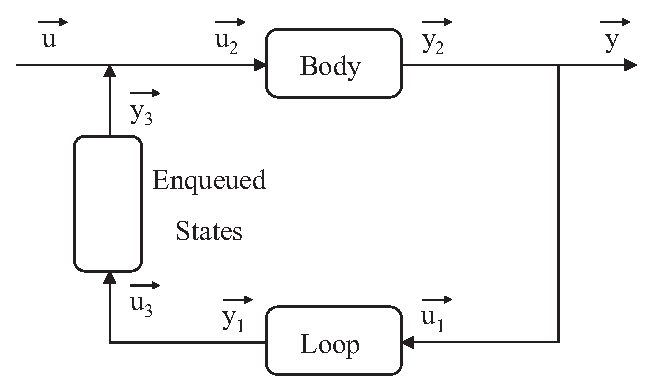
\includegraphics[width=6.0in]{figures/feedback2.eps}
  \caption{Labelled feedback loop}
  \label{fig:feedback2}
\end{figure}

    From figure \ref{fig:feedback2} it is apparent that $\vec{\mathbf{u_3}} =
\vec{\mathbf{y_1}}$, $\vec{\mathbf{y}} = \vec{\mathbf{y_2}} =
\vec{\mathbf{u_1}}$, and $\vec{\mathbf{u_2}}$ is composed of
$\vec{\mathbf{u}}$ and $\vec{\mathbf{u_3}}$. We can write the
equations for the body block as:
\begin{eqnarray*}
\vec{\dot{\mathbf{x_2}}} & = & \mathbf{A_2} \vec{\mathbf{x_2}} +
\mathbf{B_2} \vec{\mathbf{u_2}} = \mathbf{A_2}\vec{\mathbf{x_2}} +
\mathbf{B_{2\_1}} \vec{\mathbf{u}} + \mathbf{B_{2\_2}}
\vec{\mathbf{y_3}} = \mathbf{A_2}\vec{\mathbf{x_2}} +
\mathbf{B_{2\_1}} \vec{\mathbf{u}} + \mathbf{B_{2\_2}}
\mathbf{C_3} \vec{\mathbf{x_3}} \\
\vec{\mathbf{y_2}} & = & \mathbf{C_2} \vec{\mathbf{x_2}} +
\mathbf{D_2} \vec{\mathbf{u_2}} = \mathbf{C_2}\vec{\mathbf{x_2}} +
\mathbf{D_{2\_1}} \vec{\mathbf{u}} + \mathbf{D_{2\_2}}
\vec{\mathbf{y_3}} = \mathbf{C_2}\vec{\mathbf{x_2}} +
\mathbf{D_{2\_1}} \vec{\mathbf{u}} + \mathbf{D_{2\_2}}
\mathbf{C_3} \vec{\mathbf{x_3}}
\end{eqnarray*}

    Since $\vec{\mathbf{y}} = \vec{\mathbf{y_2}}$, we have written
the output of the feedback loop and the update for
$\vec{\mathbf{x_2}}$ in terms of the input to the feedback loop
and the state vectors. For the updates to $\vec{\mathbf{x_1}}$ and
$\vec{\mathbf{x_3}}$ we can write:
\begin{eqnarray*}
\vec{\dot{\mathbf{x_1}}} & = & \mathbf{A_1} \vec{\mathbf{x_1}} +
\mathbf{B_1} \vec{\mathbf{u_1}} = \mathbf{A_1}\vec{\mathbf{x_1}} +
\mathbf{B_1} \vec{\mathbf{y}} =  \mathbf{A_1}\vec{\mathbf{x_1}} +
\mathbf{B_1}(\mathbf{C_2}\vec{\mathbf{x_2}} + \mathbf{D_{2\_1}}
\vec{\mathbf{u}} + \mathbf{D_{2\_2}} \mathbf{C_3}
\vec{\mathbf{x_3}}) \\
& = & \mathbf{A_1}\vec{\mathbf{x_1}} +
\mathbf{B_1}\mathbf{C_2}\vec{\mathbf{x_2}} + \mathbf{B_1}
\mathbf{D_{2\_1}} \vec{\mathbf{u}} + \mathbf{B_1}
\mathbf{D_{2\_2}} \mathbf{C_3} \vec{\mathbf{x_3}} \\ \\
\vec{\dot{\mathbf{x_3}}} & = & \mathbf{A_3} \vec{\mathbf{x_3}} +
\mathbf{B_3} \vec{\mathbf{u_3}} = \mathbf{A_3}\vec{\mathbf{x_3}} +
\mathbf{B_3} \vec{\mathbf{y_1}} =  \mathbf{A_3}\vec{\mathbf{x_3}}
+ \mathbf{B_3}(\mathbf{C_1}\vec{\mathbf{x_1}} + \mathbf{D_1}
\vec{\mathbf{u_1}}) \\
& = & \mathbf{A_3}\vec{\mathbf{x_3}} +
\mathbf{B_3}(\mathbf{C_1}\vec{\mathbf{x_1}} +
\mathbf{D_1}\vec{\mathbf{y}}) = \mathbf{A_3}\vec{\mathbf{x_3}} +
\mathbf{B_3}(\mathbf{C_1}\vec{\mathbf{x_1}} +
\mathbf{D_1}(\mathbf{C_2}\vec{\mathbf{x_2}} + \mathbf{D_{2\_1}}
\vec{\mathbf{u}} + \mathbf{D_{2\_2}} \mathbf{C_3}
\vec{\mathbf{x_3}})) \\
& = & \mathbf{A_3}\vec{\mathbf{x_3}} +
\mathbf{B_3}\mathbf{C_1}\vec{\mathbf{x_1}} +
\mathbf{B_3}\mathbf{D_1}\mathbf{C_2}\vec{\mathbf{x_2}} +
\mathbf{B_3}\mathbf{D_1}\mathbf{D_{2\_1}} \vec{\mathbf{u}} +
\mathbf{B_3}\mathbf{D_1}\mathbf{D_{2\_2}} \mathbf{C_3}
\vec{\mathbf{x_3}}
\end{eqnarray*}

    For the input and output rates we have $o = E * w_2$
and $u = u_2$. We use the states of all three representations, so
$s = s_1 + s_2 + s_3$ and $\overrightarrow{\mathbf{initVec}} =
\left [ \begin{array} {c} \overrightarrow{\mathbf{initVec_1}} \\
\overrightarrow{\mathbf{initVec_2}} \\
\overrightarrow{\mathbf{initVec_3}} \end{array} \right ]$. For
simplicity, we do not consider a loop or body block with
initialization matrices.

\section{Representation Changes}

\subsection{Expansion}

    We may want to run a block multiple times in order to
properly combine it with other blocks. For example, suppose block
$B_1$ inputs three items and outputs two items, and block $B_2$
inputs five items and outputs seven items. In order to combine
these blocks in a pipeline, $B_1$ must run five times (in order to
output ten items) and $B_2$ must run two times (in order to input
ten items). Therefore, we need to have a method to expand a
representation so that it models a block running multiple times,
rather than once.

    Consider the state-space equation pair, where $\vec{\mathbf{u_1}}$ and
$\vec{\mathbf{y_1}}$ are the first set of inputs and outputs, and
$\vec{\mathbf{x}}$ is the original state vector:
\begin{eqnarray*}
\vec{\dot{\mathbf{x}}} & = & \mathbf{A}\vec{\mathbf{x}} + \mathbf{B}\vec{\mathbf{u_1}} \\
\vec{\mathbf{y_1}} & = & \mathbf{C}\vec{\mathbf{x}} +
\mathbf{D}\vec{\mathbf{u_1}}
\end{eqnarray*}

    If we run the block again, the equation pair in terms of the
original state vector $\vec{\mathbf{x}}$ and the next set of
inputs and outputs ($\vec{\mathbf{u_2}}$ and $\vec{\mathbf{y_2}}$)
is:
\begin{eqnarray*}
\vec{\dot{\mathbf{x}}} & = & \mathbf{A}(\mathbf{A}\vec{\mathbf{x}}
+
\mathbf{B}\vec{\mathbf{u_1}}) + \mathbf{B}\vec{\mathbf{u_2}} \\
\vec{\mathbf{y_2}} & = & \mathbf{C}(\mathbf{A}\vec{\mathbf{x}} +
\mathbf{B}\vec{\mathbf{u_1}}) + \mathbf{D}\vec{\mathbf{u_2}}
\end{eqnarray*}

Simplifying yields:
\begin{eqnarray*}
\vec{\dot{\mathbf{x}}} & = & \mathbf{A}^2\vec{\mathbf{x}} +
\mathbf{AB}\vec{\mathbf{u_1}} + \mathbf{B}\vec{\mathbf{u_2}} \\
\vec{\mathbf{y_2}} & = & \mathbf{CA}\vec{\mathbf{x}} +
\mathbf{CB}\vec{\mathbf{u_1}} + \mathbf{D}\vec{\mathbf{u_2}}
\end{eqnarray*}

    Let $\vec{\mathbf{u}}$ be the combined input vector
($\vec{\mathbf{u}} = \left [ \begin{array} {c} \vec{\mathbf{u_1}}
\\ \vec{\mathbf{u_2}} \end{array} \right ]$) and $\vec{\mathbf{y}}$ be the combined output vector
($\vec{\mathbf{y}} = \left [ \begin{array} {c} \vec{\mathbf{y_1}}
\\ \vec{\mathbf{y_2}} \end{array} \right ]$). The representation in terms of these two
vectors is:
\begin{eqnarray*}
\vec{\dot{\mathbf{x}}} & = & \mathbf{A_2}\vec{\mathbf{x}} + \mathbf{B_2}\vec{\mathbf{u}} \\
\vec{\mathbf{y}} & = & \mathbf{C_2}\vec{\mathbf{x}} + \mathbf{D_2}\vec{\mathbf{u}} \\
\mathbf{A_2} & = & \mathbf{A}^2 \\
\mathbf{B_2} & = & \left [ \begin{array} {cc} \mathbf{AB} & \mathbf{B} \end{array} \right ] \\
\mathbf{C_2} & = & \left [ \begin{array} {c} \mathbf{C} \\
\mathbf{CA} \end{array} \right ] \\
\mathbf{D_2} & = & \left [ \begin{array} {cc} \mathbf{D} & \mathbf{0} \\
\mathbf{CB} & \mathbf{D} \end{array} \right ]
\end{eqnarray*}

    This new representation corresponds to a block that upon
every execution runs the old block twice. By induction, a general
formula for running a block n times is:
\begin{eqnarray}
\mathbf{A_n} & = & \mathbf{A}^n \\
\mathbf{B_n} & = & \left [ \begin{array} {ccccc} \mathbf{A}^{n-1}
\mathbf{B} & \mathbf{A}^{n-2} \mathbf{B} & ...  & \mathbf{AB} &
\mathbf{B} \end{array} \right ] \\
\mathbf{C_n} & = & \left [ \begin{array} {c} \mathbf{C} \\
\mathbf{CA} \\
... \\
\mathbf{CA^{n-2}} \\
\mathbf{CA^{n-1}} \end{array} \right ] \\
\mathbf{D_n} & = & \left [ \begin{array} {ccccccc}
\mathbf{D} & \mathbf{0} & \mathbf{0} & ... & \mathbf{0} & \mathbf{0} & \mathbf{0} \\
\mathbf{CB} & \mathbf{D} & \mathbf{0} & ... & \mathbf{0} & \mathbf{0} & \mathbf{0} \\
\mathbf{CAB} & \mathbf{CB} & \mathbf{D} & ... & \mathbf{0} & \mathbf{0} & \mathbf{0} \\
... & ... & ... & ... & ... & ... & ... \\
\mathbf{CA}^{n-4} \mathbf{B} & \mathbf{CA}^{n-5} \mathbf{B} &
\mathbf{CA}^{n-6} \mathbf{B} & ... & \mathbf{D} & \mathbf{0} & \mathbf{0} \\
\mathbf{CA}^{n-3} \mathbf{B} & \mathbf{CA}^{n-4} \mathbf{B} &
\mathbf{CA}^{n-5} \mathbf{B} & ... & \mathbf{CB} & \mathbf{D} & \mathbf{0} \\
\mathbf{CA}^{n-2} \mathbf{B} & \mathbf{CA}^{n-3} \mathbf{B} &
\mathbf{CA}^{n-4} \mathbf{B} & ... & \mathbf{CAB} & \mathbf{CB} &
\mathbf{D} \end{array} \right ]
\end{eqnarray}

    Since initializations are not affected, $\overrightarrow{\mathbf{initVec}}$,
$\mathbf{preA}$, $\mathbf{preB}$, $stored$, and $o_{pre}$ remain
unchanged from the initial representation. Since the number of
states is not changed, $s$ remains the same. The new
representation runs the old representation $n$ times, so $u_{new}
= n * u_{old}$, $o_{new} = n * o_{old}$.

    As mentioned in the pipeline combination section, we may need
to run a block $n$ times, in addition to its initialization
matrices, for the purpose of initializing the full pipeline. We
denoted the matrices for doing this as $\mathbf{A^e}$,
$\mathbf{B^e}$, $\mathbf{C^e}$, and $\mathbf{D^e}$. If the block
being run $n$ times does not need initialization, the calculation
for these four matrices is exactly the same as described in
equations (3.2)-(3.5). Otherwise, we must make some slight
modifications:
\begin{eqnarray}
\mathbf{A^e} & = & \mathbf{A}^n \mathbf{A_{pre}} \\
\mathbf{B^e} & = & \left [ \begin{array} {ccccc} \mathbf{A^n}
\mathbf{B_{pre}} & \mathbf{A^{n-1}} \mathbf{B} & \mathbf{A^{n-2}}
\mathbf{B} & ... & \mathbf{B}
\end{array} \right ] \\
\mathbf{C^e} & = & \left [ \begin{array} {c} \mathbf{C} \mathbf{A_{pre}} \\
\mathbf{C} \mathbf{A} \mathbf{A_{pre}} \\ ... \\
\mathbf{C} \mathbf{A^{n-1}} \mathbf{A_{pre}} \end{array} \right ] \\
\mathbf{D^e} & = & \left [ \begin{array} {cccccccc} \mathbf{C}
\mathbf{B_{pre}} & \mathbf{D} & \mathbf{0} &
\mathbf{0} & ... & \mathbf{0} & \mathbf{0} \\
\mathbf{C} \mathbf{A} \mathbf{B_{pre}} & \mathbf{CB} &
\mathbf{D} & \mathbf{0} & ... & \mathbf{0} & \mathbf{0} \\
\mathbf{C} \mathbf{A}^2 \mathbf{B_{pre}} & \mathbf{CAB} &
\mathbf{CB} & \mathbf{D} & ... & \mathbf{0} & \mathbf{0} \\
... & ... & ... & ... & ... & ... \\
\mathbf{C} \mathbf{A^{n-1}} \mathbf{B_{pre}} & \mathbf{CA}^{n-2}
\mathbf{B} & \mathbf{CA}^{n-3} \mathbf{B} &
\mathbf{CA}^{n-3} \mathbf{B} & ... & \mathbf{CB} & \mathbf{D} \\
 \end{array} \right ]
\end{eqnarray}

\subsection{Increasing the number of Stored Inputs}

    As mentioned in Section 3.3.1, it may be necessary to changed the
stored inputs in a representation in order to combine it with
another representation in a pipeline. Suppose we want to change
the number of stored inputs from $oldStored$ to $newStored$.
Consider what happens in the old representation, with $oldStored$
stored input variables. The filter accesses $peek(0)$, $peek(1)$,
... $peek(oldStored-1)$ from the $oldStored$ stored input state
variables. The $o$ inputs to the filter are $peek(oldStored)$,
$peek(oldStored+1)$, ... $peek(oldStored+o-1)$. Now we want to add
$newStored-oldStored$ stored input variables, so that the total
$newStored$ stored input variables represent $peek(0)$, $peek(1)$,
... $peek(newStored-1)$, and the $o$ inputs to the filter are
$peek(newStored)$, $peek(newStored+1)$, ... $peek(newStored+o-1)$.
Therefore, any references in the original representation to
$peek(0)$, $peek(1)$, ... $peek(oldStored-1)$ remain the same,
while references to $peek(oldStored)$, $peek(oldStored)$, ...
$peek(oldStored+o-1)$ must be changed.

    The old representation was:
\begin{eqnarray*}
\left [ \begin{array} {c} \vec{\dot{\mathbf{x_1}}} \\
\vec{\dot{\mathbf{x_2}}}
\end{array} \right ] & = & \left [ \begin{array} {cc} \mathbf{A_{11}} & \mathbf{A_{12}} \\
\mathbf{A_{21}} & \mathbf{A_{22}} \end{array} \right ] \left [
\begin{array} {c} \vec{\mathbf{x_1}} \\ \vec{\mathbf{x_2}} \end{array} \right ]
 + \left [ \begin{array} {cc} \mathbf{B_{11}} & \mathbf{B_{12}} \\
\mathbf{B_{21}} & \mathbf{B_{22}} \end{array} \right ] \left[
\begin{array} {c} \vec{\mathbf{u_1}} \\ \vec{\mathbf{u_2}} \end{array} \right ] \\
\vec{\mathbf{y}} & = & \left [ \begin{array} {cc} \mathbf{C_1} &
\mathbf{C_2} \end{array} \right ] \left [
\begin{array} {c} \vec{\mathbf{x_1}} \\ \vec{\mathbf{x_2}} \end{array} \right ] +
\left [ \begin{array} {cc} \mathbf{D_1} & \mathbf{D_2}
\end{array} \right ] \left [ \begin{array} {c} \vec{\mathbf{u_1}} \\
\vec{\mathbf{u_2}} \end{array} \right ]
\end{eqnarray*}

    We have divided the state vector $\vec{\mathbf{x}}$ into the non-stored input variables ($\vec{\mathbf{x_1}}$)
and the stored input variables ($\vec{\mathbf{x_2}}$), and divided
the input vector $\vec{\mathbf{u}}$ into the first
$newStored-oldStored$ inputs ($\vec{\mathbf{u_1}}$) and the
remaining inputs ($\vec{\mathbf{u_2}}$). We will assume
$newStored-oldStored <= o$ (If not we can run this algorithm
multiple times). The matrices $\mathbf{A}$, $\mathbf{B}$,
$\mathbf{C}$, and $\mathbf{D}$ are put into block-matrix form
according to the state and input vector divisions.

    In our new representation, we use $\vec{\mathbf{x_3}}$ to denote the
added $newStored - oldStored$ states. As mentioned early,
references to the first $oldStored$ stored input states
($\vec{\mathbf{x_2}}$) remain the same. Additionally, references
to the non-input states ($\vec{\mathbf{x_1}}$) also remain the
same. Our new representation so far is:
\begin{eqnarray*}
\left [ \begin{array} {c} \vec{\dot{\mathbf{x_1}}} \\ \vec{\dot{\mathbf{x_2}}} \\
\vec{\dot{\mathbf{x_3}}}
\end{array} \right ] & = & \left [ \begin{array} {ccc} \mathbf{A_{11}} & \mathbf{A_{12}} & ? \\
\mathbf{A_{21}} & \mathbf{A_{22}} & ? \\ ? & ? & ?
\end{array} \right ] \left [
\begin{array} {c} \vec{\mathbf{x_1}} \\ \vec{\mathbf{x_2}} \\ \vec{\mathbf{x_3}} \end{array} \right ]
 + \left [ \begin{array} {cc} ? & ? \\ ? & ? \\ ? & ? \end{array} \right ] \left[
\begin{array} {c} \vec{\mathbf{u_1}} \\ \vec{\mathbf{u_2}} \end{array} \right ] \\
\vec{\mathbf{y}} & = & \left [ \begin{array} {ccc} \mathbf{C_1} &
\mathbf{C_2} & ? \end{array} \right ] \left [
\begin{array} {c} \vec{\mathbf{x_1}} \\ \vec{\mathbf{x_2}} \\ \vec{\mathbf{x_3}} \end{array} \right ] +
\left [ \begin{array} {cc} ? & ?
\end{array} \right ] \left [ \begin{array} {c} \vec{\mathbf{u_1}} \\
\vec{\mathbf{u_2}} \end{array} \right ]
\end{eqnarray*}

    The ? indicates yet to be determined entries. In the old
representation, the first $newStored-oldStored$ input elements
($u_1$) were $peek(oldStored)$ ... $peek(newStored-1)$. In the new
representation, these values are stored as states ($x_3$).
Therefore, any matrix block that was previously multiplied by
$u_1$ should be multiplied by $x_2$ instead. Now the new
representation is:
\begin{eqnarray*}
\left [ \begin{array} {c} \vec{\dot{\mathbf{x_1}}} \\ \vec{\dot{\mathbf{x_2}}} \\
\vec{\dot{\mathbf{x_3}}}
\end{array} \right ] & = & \left [ \begin{array} {ccc} \mathbf{A_{11}} &
\mathbf{A_{12}} & \mathbf{B_{11}} \\ \mathbf{A_{21}} &
\mathbf{A_{22}} & \mathbf{B_{21}} \\ ? & ? & ?  \end{array} \right
] \left [
\begin{array} {c} \vec{\mathbf{x_1}} \\ \vec{\mathbf{x_2}} \\ \vec{\mathbf{x_3}} \end{array} \right ]
 + \left [ \begin{array} {cc} ? & ? \\ ? & ? \\ ? & ? \end{array} \right ] \left[
\begin{array} {c} \vec{\mathbf{u_1}} \\ \vec{\mathbf{u_2}} \end{array} \right ] \\
\vec{\mathbf{y}} & = & \left [ \begin{array} {ccc} \mathbf{C_1} &
\mathbf{C_2} & \mathbf{D_1}  \end{array} \right ] \left [
\begin{array} {c} \vec{\mathbf{x_1}} \\ \vec{\mathbf{x_2}} \\ \vec{\mathbf{x_3}} \end{array} \right ] +
\left [ \begin{array} {cc} ? & ?
\end{array} \right ] \left [ \begin{array} {c} \vec{\mathbf{u_1}} \\
\vec{\mathbf{u_2}} \end{array} \right ]
\end{eqnarray*}

    In the old representation, the remaining $o-(newStored-oldStored)$ input elements
($u_2$) were $peek(newStored)$ ... $peek(o+oldStored-1)$. In the
new representation, these are the first $o-(newStored-oldStored)$
input elements. We divide the input vector into the first
$o-(newStored-oldStored)$ elements ($\vec{u_{1'}}$) and the
remaining $newStored-oldStored$ elements ($\vec{u_{2'}}$). Any
matrix block that was previously multiplied by
$\vec{\mathbf{u_2}}$ should be multiplied by $\vec{u_{1'}}$
instead. Additionally, there is no dependence on $\vec{u_{2'}}$ by
$\vec{\mathbf{x_1}}$, $\vec{\mathbf{x_2}}$, or $\vec{\mathbf{y}}$.
The new representation is:
\begin{eqnarray*}
\left [ \begin{array} {c} \vec{\dot{\mathbf{x_1}}} \\ \vec{\dot{\mathbf{x_2}}} \\
\vec{\dot{\mathbf{x_3}}} \end{array} \right ] & = & \left [
\begin{array} {ccc} \mathbf{A_{11}} & \mathbf{A_{12}} &
\mathbf{B_{11}} \\ \mathbf{A_{21}} & \mathbf{A_{22}} &
\mathbf{B_{21}} \\ ? & ? & ? \end{array} \right ] \left [
\begin{array} {c} \vec{\mathbf{x_1}} \\ \vec{\mathbf{x_2}} \\ \vec{\mathbf{x_3}} \end{array} \right ]
+ \left [ \begin{array} {cc} \mathbf{B_{12}} & \mathbf{0} \\
\mathbf{B_{22}} & \mathbf{0} \\ ? & ? \end{array} \right ] \left[
\begin{array} {c} \vec{u_{1'}} \\ \vec{u_{2'}} \end{array} \right ] \\
\vec{\mathbf{y}} & = & \left [ \begin{array} {ccc} \mathbf{C_1} &
\mathbf{C_2} & \mathbf{D_1} \end{array} \right ] \left [
\begin{array} {c} \vec{\mathbf{x_1}} \\ \vec{\mathbf{x_2}} \\ \vec{\mathbf{x_3}} \end{array} \right ] +
\left [ \begin{array} {cc} \mathbf{D_2} & \mathbf{0}
\end{array} \right ] \left [ \begin{array} {c} \vec{u_{1'}} \\
\vec{u_{2'}} \end{array} \right ]
\end{eqnarray*}

    The entries for the state update $\vec{\dot{\mathbf{x_3}}}$ remain to be
determined. Any stored input variable representing $peek(i)$ must
get updated by $peek(i+o)$. $\vec{\dot{\mathbf{x_3}}}$ is
$peek(oldStored)$ ... $peek(newStored-1)$, so it must be updated
by $peek(o+oldStored)$ ... $peek(o+newStored-1)$. This is
precisely $\vec{u_{2'}}$, so the final new representation is:
\begin{eqnarray*}
\left [ \begin{array} {c} \vec{\dot{\mathbf{x_1}}} \\ \vec{\dot{\mathbf{x_2}}} \\
\vec{\dot{\mathbf{x_3}}}
\end{array} \right ] & = & \left [ \begin{array} {ccc} \mathbf{A_{11}} &
\mathbf{A_{12}} & \mathbf{B_{11}} \\ \mathbf{A_{21}} &
\mathbf{A_{22}} & \mathbf{B_{21}} \\ \mathbf{0} & \mathbf{0} & \mathbf{0} \\
\end{array} \right ] \left [ \begin{array} {c} \vec{\mathbf{x_1}} \\ \vec{\mathbf{x_2}} \\
\vec{\mathbf{x_3}} \end{array} \right ] + \left [ \begin{array}
{cc} \mathbf{B_{12}} & \mathbf{0} \\ \mathbf{B_{22}} & \mathbf{0} \\ \mathbf{0} & \mathbf{I} \\
\end{array} \right ] \left[ \begin{array} {c} \vec{u_{1'}} \\ \vec{u_{2'}} \end{array} \right ] \\
\vec{\mathbf{y}} & = & \left [ \begin{array} {ccc} \mathbf{C_1} &
\mathbf{C_2} & \mathbf{D_1} \end{array} \right ] \left [
\begin{array} {c} \vec{\mathbf{x_1}} \\ \vec{\mathbf{x_2}} \\ \vec{\mathbf{x_3}} \end{array} \right ] +
\left [ \begin{array} {cc} \mathbf{D_2} & \mathbf{0}
\end{array} \right ] \left [ \begin{array} {c} \vec{u_{1'}} \\
\vec{u_{2'}} \end{array} \right ]
\end{eqnarray*}

    Similarly, let the original initialization equation be:
\begin{eqnarray*}
\left [ \begin{array} {c} \vec{\dot{\mathbf{x_1}}} \\
\vec{\dot{\mathbf{x_2}}} \end{array} \right ] = \left [
\begin{array} {cc} \mathbf{A_{pre11}} & \mathbf{A_{pre12}} \\
\mathbf{0} & \mathbf{0} \end{array} \right ] \left [
\begin{array} {c} \vec{\mathbf{x_1}} \\ \vec{\mathbf{x_2}}
\end{array} \right ] + \left [ \begin{array} {cc} \mathbf{B_{pre11}} & \mathbf{B_{pre12}} \\
\mathbf{I} & \mathbf{0} \end{array} \right ] \left [ \begin{array}
{c} \vec{\mathbf{u_{pre1}}} \\ \vec{\mathbf{u_{pre2}}}
\end{array} \right ]
\end{eqnarray*}

    Where $\vec{\mathbf{u_{pre1}}}$ has length $oldStored$, and
$\vec{\mathbf{u_{pre2}}}$ has length $o_{pre} - oldStored$. Now we
simply consider $\vec{\mathbf{u_{pre1}}}$ to have length
$newStored$ and $\vec{\mathbf{u_{pre2}}}$ to have length $o_{pre}
- newStored$. If $o_{pre} < newStored$, we set $o_{pre} =
newStored$. Then the initialization equation is the same as
before, except the original stored input states
($\vec{\mathbf{x_2}})$ are replaced by the new stored input states
($\left [ \begin{array} {c} \vec{\mathbf{x_2}} \\
\vec{\mathbf{x_3}} \end{array} \right ]$).

    We have derived $\mathbf{A}$, $\mathbf{B}$, $\mathbf{C}$, $\mathbf{D}$,
$\mathbf{A_{pre}}$, and $\mathbf{B_{pre}}$ for the new
representation. Clearly, $stored = newStored$ and $o_{pre} =
o_{preold} + newStored-oldStored$. The input/output rate remains
the same, so $o = o_{old}$ and $u = u_{old}$. We have added
$newStored-oldStored$ total states, so $s = s_{old} + (newStored -
oldStored)$ and $\overrightarrow{\mathbf{initVec}} =
\left [ \begin{array} {c} \overrightarrow{\mathbf{initVec_1}} \\
\overrightarrow{\mathbf{initVec_2}} \\ \overrightarrow{\mathbf{0}}
\end{array} \right ]$.

\section{Replacement}

    Once we have combined filters to a single representation and
performed optimizations on it (see Chapter 4), we would like to
convert it to StreamIt code. Given a representation $\mathrm{R}$
we can create the following StreamIt filter:

\begin{scriptsize}
\begin{verbatim}
float -> float filter replacementFilter() {
  float x0, ... , x{s-1};

  prework push 0 pop preu peek preu {
    x0 = preA[0,0]*x0 + ... + preA[0,s-1]*x{s-1} + preB[0,0]*peek(0) + ... + preB[0,preu-1]*peek(preu-1);
    x1 = preA[1,0]*x0 + ... + preA[1,s-1]*x{s-1} + preB[1,0]*peek(0) + ... + preB[1,preu-1]*peek(preu-1);
    ...
    x{s-1} = preA[s-1,0]*x0 + ... + preA[s-1,s-1]*x{s-1} + preB[s-1,0]*peek(0) + ... + preB[s-1,preu-1]*peek(preu-1);
  }

  work push u pop o peek o {
    float x0_temp, ... , x{s-1}_temp;

    push(C[0,0]*x0 + ... + C[0,s-1]*x{s-1} + D[0,0]*peek(0) + ... + D[0,o-1]*peek(o-1));
    push(C[1,0]*x0 + ... + C[1,s-1]*x{s-1} + D[1,0]*peek(0) + ... + D[1,o-1]*peek(o-1));
    ...
    push(C[u,0]*x0 + ... + C[u,s-1]*x{s-1} + D[u,0]*peek(0) + ... + D[u,o-1]*peek(o-1));

    x0_temp = A[0,0]*x0 + ... + A[0,s-1]*x{s-1} + B[0,0]*peek(0) + ... + B[0,o-1]*peek(o-1);
    x1_temp = A[1,0]*x0 + ... + A[1,s-1]*x{s-1} + B[1,0]*peek(0) + ... + B[1,o-1]*peek(o-1);
    ...
    x{s-1}_temp = A[s-1,0]*x0 + ... + A[s-1,s-1]*x{s-1} + B[s-1,0]*peek(0) + ... + B[s-1,o-1]*peek(o-1);

    x0 = x0_temp;
    ...
    x{s-1} = x{s-1}_temp;

    pop(); pop(); ... pop(); // o pops
  }
}
\end{verbatim}
\end{scriptsize}

    We make two modifications to this filter. If a matrix entry is
zero, any term involving that matrix entry is not placed in the
filter. If a matrix entry is one, the multiplication of a peek or
variable by this matrix entry is removed.

\chapter{Optimization}

     There are multiple metrics used to analyze performance
of a computer program - speed (throughput, or outputs per second),
space, power consumption, etc. We focus on speed and attempt to
minimize the computation performed to produce each output.
Obviously, this type of optimization has positive effects on the
other parameters. However, we are mainly concerned with speed
because it is simple to track, and due to falling hardware costs,
is frequently a program's bottleneck.

    There are two types of optimizations we consider.  The first is to
remove extraneous state variables from the linear state-space
representation. This reduces the memory allocation for a program
and reduces the number of loads and stores executed, which are
typically time intensive operations. It also eliminates
computations that involve the removed states.  The second
optimization is to reduce the parametrization of a state-space
representation, by changing the representation to one with more
zero and one entries in its matrices. This directly eliminates
computations, since all multiplications by zero or one are not
processed by the replacement algorithm.

\section{State-Space Transformations}

    For any state-space equation pair, there are an infinite
number of transformations to an equivalent state-space system.
These transformations involve a change of basis of the state
vector $\vec{\mathbf{x}}$ to $\mathbf{T} \vec{\mathbf{x}}$, where
$\mathbf{T}$ is an invertible matrix. Consider the state-update
equation $\vec{\dot{\mathbf{x}}} = \mathbf{A} \vec{\mathbf{x}} +
\mathbf{B} \vec{\mathbf{u}}$. Multiplying the entire equation by
$\mathbf{T}$ yields:
\begin{eqnarray*}
\mathbf{T} \vec{\dot{\mathbf{x}}} = \mathbf{TA} \vec{\mathbf{x}} +
\mathbf{TB} \vec{\mathbf{u}}
\end{eqnarray*}

    Since $\mathbf{T}^{-1} \mathbf{T} = \mathbf{I}$, we can write:
\begin{eqnarray*}
\mathbf{T} \vec{\dot{\mathbf{x}}} & = & \mathbf{TA}
(\mathbf{T}^{-1} \mathbf{T}) \vec{\mathbf{x}} + \mathbf{TB}
\vec{\mathbf{u}} = \mathbf{TA}
\mathbf{T}^{-1} (\mathbf{T} \vec{\mathbf{x}}) + \mathbf{TB} \vec{\mathbf{u}} \\
\vec{\mathbf{y}} & = & \mathbf{C} (\mathbf{T}^{-1} \mathbf{T})
\vec{\mathbf{x}} + \mathbf{D} \vec{\mathbf{u}} = \mathbf{C}
\mathbf{T}^{-1} (\mathbf{T} \vec{\mathbf{x}}) + \mathbf{D}
\vec{\mathbf{u}}
\end{eqnarray*}

    Where we have introduced the output equation as well. Let
$\vec{\mathbf{z}} = \mathbf{T} \vec{\mathbf{x}}$.
$\vec{\mathbf{z}}$ is a new state vector related to the old state
vector $\vec{\mathbf{x}}$ by the change of basis $\mathbf{T}$.
Substituting into the equations above we get:
\begin{eqnarray*}
\vec{\dot{\mathbf{z}}} & = & \mathbf{TA} \mathbf{T}^{-1} \vec{\mathbf{z}} + \mathbf{TB} \vec{\mathbf{u}} \\
\vec{\mathbf{y}} & = & \mathbf{C} \mathbf{T}^{-1}\vec{\mathbf{z}}
+ \mathbf{D}\vec{\mathbf{u}}
\end{eqnarray*}

    These is precisely the original state-space equation pair,
with $\mathbf{A}$, $\mathbf{B}$, and $\mathbf{C}$ transformed to
$\mathbf{T} \mathbf{A} \mathbf{T}^{-1}$, $\mathbf{T} \mathbf{B}$,
and $\mathbf{C} \mathbf{T}^{-1}$, respectively.

    For a StreamIt state-space representation $\mathrm{R}$, we must
determine how the other values change. The initialization state
update equation is essentially the same as the regular state
update equation, so $\mathbf{A_{pre}}$ and $\mathbf{B_{pre}}$ are
transformed to $\mathbf{T} \mathbf{A_{pre}} \mathbf{T}^{-1}$ and
$\mathbf{T} \mathbf{B}$ respectively. Since the old state vector
$\vec{\mathbf{x}}$ is multiplied by $\mathbf{T}$, the old initial
state vector is multiplied by $\mathbf{T}$. The number of states,
inputs, and outputs is the same, so $s$, $o$, and $u$ are
unchanged.

\section{State Removal}

    There are two types of states that can be removed from a state-space system
without changing its behavior - unreachable and unobservable
states. Informally, unreachable states are unaffected by inputs
and unobservable states have no effect on outputs. More formally,
the set of states in a system can be divided into reachable and
unreachable states where:
\begin{enumerate}
\item The unreachable states are not updated by any of the
reachable states.

\item The unreachable states are not updated by any inputs.
\end{enumerate}

    In terms of the state-space equation pair, this means $\mathbf{A}[i,j] =
0, \mathbf{B}[i,k] = 0$ where $i$ is the row of an unreachable
state, $j$ is the column of a reachable state, and $k$ is any of
the inputs.
    If all the unreachable states are initially zero, they
remain zero because they are not updated by a non-zero value
(either a reachable state or an input). Therefore, all unreachable
states that are not initialized can be removed from a
representation, since they do not effect the reachable states or
the outputs.

    The set of states in a system can also be divided into
observable and unobservable states where:
\begin{enumerate}
\item The observable states are not updated by any of the
unobservable states.

\item The outputs do not depend on the unobservable states.
\end{enumerate}

    In terms of the state-space equation pair, this means $\mathbf{C}[i,j] =
0, \mathbf{D}[k,j] = 0$ where $j$ is the column of an observable
state, $i$ is the row of an unobservable state, and $k$ is any of
the outputs.
    The unobservable states are not used to update the observable
states and are not used to determine the outputs. Therefore, all
unobservable states can be removed from a representation
(regardless of their initial values).

    A simple algorithm to isolate the unreachable and unobservable
states in a system by use of transformations is explained in
\cite{Mayne}. The algorithm works as follows: Perform row
operations on the augmented matrix $\left [ \begin{array} {cc}
\mathbf{A} & \mathbf{B} \end{array} \right ]$ to put it into a
type of row-echelon form\footnote{A matrix is in standard
row-echelon form if the first non-zero entry in each row is a 1
(called the leading 1) and the leading 1 in a higher row is to the
left of the leading 1 in a lower row. For our type of row-echelon
form, the \emph{last} non-zero entry in each row is a 1 (call it
the ending 1) and the ending 1 in a higher row is to the left of
the ending 1 in a lower row.}, and perform the corresponding
inverse column operations on $\mathbf{A}$ and $\mathbf{C}$ to keep
the system equivalent to the original (Performing a row operation
on a matrix is equivalent to left multiplying it by some
invertible matrix, and performing a column operation on a matrix
is equivalent to right multiplying it by some invertible matrix).
Once the augmented matrix is in the desired form, row $i$ of the
combined matrix represents an unreachable state if there are no
non-zero entries past the $i^{th}$ column. For unobservable
states, the combined matrix $\left [ \begin{array} {cc}
\mathbf{A}^T & \mathbf{C}^T
\end{array} \right ]$ is operated on instead.

    Using this algorithm, we can find the entire set of unobservable
states and remove them all. The only exceptions are those
unobservable states that affect observable states in the
initialization matrix $\matrix{A_{pre}}$. If $j$ is the column of
an observable state then we must have $\mathbf{A_{pre}}[i,j] = 0$
for all values of $i$, where $i$ is the row of an observable
state. Otherwise, the unobservable state $j$ cannot be removed,
because it affects at least one observable state, and therefore
may affect the outputs.

    More care must be taken when removing unreachable states. If an
unreachable state has a non-zero starting value, or is affected by
the initialization matrices, it cannot be removed. In either of
these cases, the unreachable state may attain a non-zero value,
and therefore may have an affect on the reachable states and/or
outputs. Additionally, an unreachable state $x_1$ that is updated
by a different unreachable state $x_2$ that cannot be removed may
eventually have a non-zero value, even if it ($x_1$) is initially
zero. Therefore, the unreachable state $x_1$ cannot be removed as
well.

    The last case may cause problems when trying to remove
unreachable states. If an unreachable state $x_1$ is updated by
unreachable states $x_2$ and $x_3$, we must check if those states
can be removed before determining if state $x_1$ can be removed.
If one of those states, say $x_2$, depends on $x_1$, we must
determine if $x_1$ can be removed before determining whether $x_2$
can be removed - resulting in an impossible `loop-like'
determination. Clearly, a more robust approach is necessary.

    Suppose we have found the set of unreachable states and they
form the first $k$ states of the state vector (we can do both of
these steps by isolating the unreachable states, then moving them
to the top of the state vector if necessary). Consider the
sub-matrix $\mathbf{A}[1:k;1:k]$ consisting of the first k rows
and first k columns of $\mathbf{A}$. This sub-matrix represents
how the unreachable states are updated based on each other.
Suppose this sub-matrix is in upper-triangular form, which means
that all entries below the main diagonal are zero. We can remove
states in the following manner:
\begin{enumerate}
\item Check the states in reverse order, from state $k$ to state
$1$.

\item For the $i^{th}$ state, check whether the state has an
initial value, is updated by the initialization matrices, or
depends on a state with a higher index. If any of these are true,
we cannot remove the state. Otherwise, we can remove the state.
\end{enumerate}

    Since the unreachable state sub-matrix is in upper-triangular
form, all unreachable states can only have dependencies on states
with a higher index. Furthermore, since we are working from the
state with highest index first, at each step in the algorithm we
can immediately determine whether or not a given state is
removable. Therefore we have found our robust approach to remove
unreachable states. What remains to be done is transforming the
sub-matrix to upper-triangular form.

    The QR algorithm, described in \cite{Trefethen}, is an iterative method of
converting any square matrix $\mathbf{P}$ to upper-triangular
form. The algorithm is essentially the following two step
procedure, applied as many times as necessary.
\begin{enumerate}
\item $\mathbf{Q} \mathbf{R} = \mathbf{P}$   (QR factorization of
P)

\item $\mathbf{P} = \mathbf{R} \mathbf{Q}$
\end{enumerate}

    The QR factorization of a matrix $\mathbf{P}$ factors
$\mathbf{P}$ into the product of an orthogonal matrix
$\mathbf{Q}$\footnote{An orthogonal matrix has the property that
its transpose is equal to its inverse} and an upper-triangular
matrix $\mathbf{R}$. Since $\mathbf{R} = \mathbf{Q}^{-1}
\mathbf{P}$, the QR algorithm is repeatedly transforming
$\mathbf{P}$ to $\mathbf{Q}^{-1} \mathbf{P} \mathbf{Q}$.

    Since $\mathbf{Q}$ is invertible, we can apply this
transformation to the unreachable state sub-matrix, where the
transformation matrix $\mathbf{T}$ is $\mathbf{Q}^{-1}$. Since we
want to keep the other states unchanged, the full transformation
matrix applied to $\mathbf{A}$, $\mathbf{B}$, $\mathbf{C}$ is
$\mathbf{T} = \left [ \begin{array} {cc} \mathbf{Q}^{-1} &
\mathbf{0} \\ \mathbf{0} & \mathbf{I} \end{array} \right ]$

\section{Putting Inputs into States}

    So far we have considered optimizations that affect $\mathbf{A}$,
$\mathbf{B}$, and $\mathbf{C}$. Since the optimizations are
entirely the result of state transformations, they do not affect
$\mathbf{D}$, which is independent of the choice of state-space
basis. By storing every input as a state, however, all the entries
of $\mathbf{D}$ are moved into $\mathbf{A}$ and can then be
changed by state optimizations.

    We have already discussed how to store inputs as states. When
every input is stored as a state, we find the new state-equation
pair is:
\begin{eqnarray*}
\left [ \begin{array} {c} \vec{\dot{\mathbf{x}}} \\
\vec{\dot{\mathbf{x_{inputs}}}} \end{array} \right ] & = & \left [
\begin{array} {cc} \mathbf{A} & \mathbf{B} \\ \mathbf{0} &
\mathbf{0} \end{array} \right ] \left [ \begin{array} {c}
\vec{\mathbf{x}} \\ \vec{\mathbf{x_{inputs}}} \end{array} \right ]
+ \left [ \begin{array} {c} \mathbf{0} \\ \mathbf{I} \end{array}
\right ] \vec{\mathbf{u}} \\
\vec{\mathbf{y}} & = & \left [ \begin{array} {cc} \mathbf{C} &
\mathbf{D} \end{array} \right ] \left [ \begin{array} {c}
\vec{\mathbf{x}} \\ \vec{\mathbf{x_{inputs}}} \end{array} \right ]
+ \mathbf{0} \vec{\mathbf{u}}
\end{eqnarray*}

    These states should be added before state-removal is
performed. It may seem counter-intuitive that we first add states,
then seek to remove them. However, the added states represent
computations involving $\mathbf{D}$, which were not considered
before. Removing some of these states results in reducing
computations involving $\mathbf{D}$.

\section{Parameter Reduction}

    After removing as many states as possible, including input
states, we want to change the state-space system to one with the
fewest number of non-zero, non-one entries (termed parameters). If
$\mathbf{A}$, $\mathbf{B}$, and $\mathbf{C}$ are completely
filled, there are $s*(s+o+u)$ parameters. Ackermann and Bucy
\cite{Ackermann/Bucy} show a general form for $\mathbf{A}$ and
$\mathbf{C}$ ($\mathbf{B}$ can be filled with parameters) to have
at most $s*(o+u)$ parameters, assuming there are no unobservable
or unreachable states. They derive this form using system impulse
responses. We will achieve this same form using row operations on
the augmented matrix $\left [
\begin{array} {cc} \mathbf{A}^T & \mathbf{C}^T \end{array} \right
]$. The form we want is:
\begin{eqnarray*}
\mathbf{A}^T & = & \left [ \begin{array} {ccccc} \mathbf{L_1} &
\mathbf{A_{12}} & \mathbf{A_{13}} & ... & \mathbf{A_{1u}} \\
\mathbf{0} & \mathbf{L_2} & \mathbf{A_{23}} & ... &
\mathbf{A_{2u}} \\ \mathbf{0} & \mathbf{0} & \mathbf{L_3} & ... &
\mathbf{A_{3u}} \\ ... & ... & ... & ... & ... \\ \mathbf{0} &
\mathbf{0} & \mathbf{0} & ... & \mathbf{L_u} \end{array} \right ] \\
\mathbf{C}^T & = & \left [ \begin{array} {ccccc} 1 & 0 & 0 & ... &
0 \\ 0 & 0 & 0 & ... & 0 \\ ... & ... & ... & ... & ... \\ 0 & 1 &
0 & ... & 0 \\ 0 & 0 & 0 & 0 & 0 \\ ... & ... & ... & ... & ... \\
0 & 0 & 0 & ... & 1 \end{array} \right ]
\end{eqnarray*}

    The matrices $\mathbf{L_i}$ are rectangular, and the matrices
$\mathbf{A_{ij}}$ are square, but do not necessarily have the same
dimensions as each other. These matrices have the form:
\begin{eqnarray*}
\mathbf{L_i} & = & \left [ \begin{array} {ccccc} 0 & 0 & ...
& 0 & * \\ 1 & 0 & ... & 0 & * \\ 0 & 1 & ... & 0 & * \\
... & ... & ... & ... & ... \\ 0 & 0 & ... & 1 & * \end{array}
\right ] \\
\mathbf{A_{ij}} & = & \left [ \begin{array} {cccc} 0 & 0 & ... & *
\\ ... & ... & ... & ... \\ 0 & 0 & ... & * \end{array} \right ]
\end{eqnarray*}

    The entries marked with a * are the parameters of the system.
This is known as the observable canonical form of the system. In
contrast, the reachable canonical form defines $\mathbf{A}$ and
$\mathbf{B}$ instead of $\mathbf{A}^T$ and $\mathbf{C}$, and
$\mathbf{C}$ may be filled with parameters instead of
$\mathbf{B}$.

    We present a simple algorithm, in pseudocode to attain the form
above. We do not include the necessary inverse column operations
that must go with all row operations.

\begin{scriptsize}
\begin{verbatim}
Reduce Parameters {
  currRow = 0; colA = 0; colC = 0;

  while(currRow < totalRows) {

   -find a non-zero entry in column colC at or below row currRow of C{transpose}, and swap it with the
    entry in row currRow;
   -set C{transpose}[currRow,colC] = 1 by scaling the row appropriately;
    make all entries above and below it zero by adding appropriate multiple of row currRow to other rows;

    currRow = currRow + 1;
    colC = colC + 1;

    do {
     -find a non-zero entry in column colA at or below row currRow of A{transpose}, and swap it with the
      entry in row currRow;
     -set A{transpose}[currRow,colA] = 1 by scaling the row appropriately;
      make all entries below it zero by adding appropriate multiple of row currRow to other rows;

      currRow = currRow + 1;
      colA = colA + 1;
    } while a non-zero entry in column colA is found

    colA = colA + 1;
  }
}
\end{verbatim}
\end{scriptsize}

    It is possible that one type of form has fewer parameters than the
other. Therefore, we perform the above algorithm on $\left [
\begin{array} {cc} \mathbf{A}^T & \mathbf{C}^T
\end{array} \right ]$ as noted to produce the observable form, and on $\left [
\begin{array} {cc} \mathbf{A} & \mathbf{B} \end{array} \right
]$ to produce the reachable form, and check which one has fewer
parameters.

\section{Staged Execution}

    Using input state variables corresponds to executing a state-space
block in two stages:
\begin{enumerate}
\item Put inputs into input state variables.

\item Execute the original block, using input states instead of
actual inputs.
\end{enumerate}

    We can add additional stages by having multiple sets of input
states - $\vec{\mathbf{x_{inputs1}}}$,
$\vec{\mathbf{x_{inputs2}}}$, etc. The first set gets saved in the
second set, the second set gets saved in the third set, etc.
Suppose there are $k$ input sets. We can write our state-space
equation pair as follows:
\begin{eqnarray*}
\left [ \begin{array} {c} \vec{\dot{\mathbf{x}}} \\ \vec{\dot{\mathbf{x_{inputsk}}}} \\
... \\ \vec{\dot{\mathbf{x_{inputs2}}}} \\
\vec{\dot{\mathbf{x_{inputs1}}}}
\end{array} \right ] & = & \left [ \begin{array} {ccccc}
\mathbf{A} & \mathbf{B} & \mathbf{0} & ... &
\mathbf{0} \\ \mathbf{0} & \mathbf{0} & \mathbf{I} & ... & \mathbf{0} \\
... & ... & ... & ... & ... \\ \mathbf{0} & \mathbf{0} &
\mathbf{0} & ... & \mathbf{I} \\ \mathbf{0} & \mathbf{0} &
\mathbf{0} & ... & \mathbf{0} \end{array} \right ] \left [
\begin{array} {c} \vec{\mathbf{x}} \\ \vec{\mathbf{x_{inputsk}}} \\ ...
\\ \vec{\mathbf{x_{inputs2}}} \\ \vec{\mathbf{x_{inputs1}}} \end{array} \right ]
+ \left [ \begin{array} {c} \mathbf{0} \\ \mathbf{0} \\ ... \\
\mathbf{0} \\ \mathbf{I} \end{array} \right ]
\vec{\mathbf{u}} \\
\vec{\mathbf{y}} & = & \left [ \begin{array} {ccccc} \mathbf{C} &
\mathbf{D} & ... & \mathbf{0} & \mathbf{0} \end{array} \right ]
\left [ \begin{array} {c} \vec{\mathbf{x}}
\\ \vec{\mathbf{x_{inputsk}}} \\ ... \\ \vec{\mathbf{x_{inputs2}}}
\\ \vec{\mathbf{x_{inputs1}}} \end{array} \right ] + \mathbf{0} \vec{\mathbf{u}}
\end{eqnarray*}

    By itself, executing the work of a filter in stages does not
result in any gain in performance. However, minimally
parameterizing the resulting system may be more productive than
minimally parameterizing the one or two execution stage system.
The canonical forms of the previous section do not in general
minimally parameterize the system; hence evaluating staged
execution remains an area of future research.

\chapter{Dynamic Scheduling Using the Runtime Library}\label{ch:ds}

The dynamic scheduler is implemented as a layer on top of the runtime library. Like the library, it is designed for but not specific to StreamIt: it can schedule any acyclic stream graph where all filters have static rates, subject to some additional limitations.\footnote{The dynamic scheduler places a maximum limit on the degree of any node in the stream graph.} A StreamIt program can be converted filter-by-filter into input to the dynamic scheduler, or a compiler can first perform high-level optimizations that modify the original stream graph.

We first discuss the advantages offered by a dynamic scheduling approach in section~\ref{ch:ds:bg} before discussing the interface and implementation of the actual scheduler in sections~\ref{ch:ds:ui} and \ref{ch:ds:imp}.

\section{Dynamic Scheduling vs. Static Scheduling}\label{ch:ds:bg}

For stream graphs that are ``well-behaved'', dynamic scheduling generally does not present any advantages over static scheduling. Dynamic scheduling inevitably involves additional communication and scheduling overhead due to extra filter loading and unloading, buffer management, and scheduling computation. When all filters in a program are data-parallel, a static scheduler can make full use of all SPEs by simply executing each filter in turn on all SPEs, with a sufficient coarsening of the steady state to amortize filter load/unload and SPE synchronization overhead. The optimal situation results when the compiler can fuse all filters into a single data-parallel filter; this produces the minimum possible communication.

Even when filters are stateful and thus cannot be data-parallelized, static software pipelining techniques~\cite{asplos06} can make full use of SPEs when the compiler has an accurate static work estimator and can divide filters in a steady state evenly across SPEs.\footnote{A single stateful filter with a heavily imbalanced work function creates a bottleneck, but dynamic schedulers are also faced with this problem.} In addition, no ``unpredictable'' cache misses or lengthy communication delays that can skew a static work estimate are possible on the Cell architecture.

Dynamic scheduling becomes beneficial when filters are not ``well-behaved'': when it is difficult to statically balance load across SPEs, difficult to estimate the amount of work done by filter work functions, or work functions perform widely varying amounts of work through the execution of the program. In these situations, dynamic scheduling may be able to deliver better load-balancing than static scheduling.

A dynamically scheduled program can be run on varying numbers of processors without requiring recompilation or the reanalysis that complex static schedulers would need to perform, and is also tolerant of changes in the availability of processors while the program is running. In addition, for stream graphs that contain filters with dynamic rates, it may not be possible to statically predict how many times filters will be run, and the balance of work in the stream graph may change as the program is run. In this case, only dynamic scheduling is able to shift workload to different portions of the stream graph as needed.\footnote{However, the current dynamic scheduler implementation does not support dynamic rates.}

\section{User Interface}\label{ch:ds:ui}

The user provides as input to the dynamic scheduler a complete description of the stream graph, specifying filters and the channels that connect them. Rates for all filters must be specified. Duplicate splitters can be handled by setting parameters of channels; round-robin splitters and joiners must be defined as separate filters.

\section{Implementation}\label{ch:ds:imp}

The Cell architecture's communication network provides very high memory bandwidth. The design of the dynamic scheduler assumes that memory will never be a bottleneck (a hypothesis that was confirmed by experiments; see chapter~\ref{ch:perf}), and the dynamic scheduler buffers all output produced on SPEs to memory. The scheduler performs dynamic course-grained software pipelining on the stream graph; if sufficient data can be buffered in all channels at all times, pipeline stalls can be avoided and all SPEs can be fully utilized. While SPE--SPE communication is more efficient than SPE--memory communication, SPE local store is generally too limited to store the buffering needed for software pipelining, and thus the scheduler never executes SPE--SPE pipelines; this avoids having to deal with work imbalances between pairs of adjacent filters. At any time, any two SPEs will typically be operating on data from widely separated iterations of the program.

At startup, the dynamic scheduler allocates a large\footnote{1 MB in the current implementation, but this can be adjusted.} buffer in memory for each channel; this is used to buffer the output of the upstream filter to provide input for the downstream filter. At any time, for any specific filter, the amount of data available in its input channels and amount of space available in its output channels, along with its rates, determines the maximum number of iterations that the filter can be run for.

The scheduler selects filters to run on SPEs based on a metric computed from the maximum number of iterations and certain filter properties (see below). When a filter is selected to run on an SPE, it is scheduled for a limited but fairly large number of iterations in order to amortize the cost of loading it. Filters run for their entire allotment of iterations; however, allotments are kept small to allow the scheduler to quickly schedule another filter if necessary in response to the changing state in the stream graph.

A replacement filter for an SPE is selected when the current filter scheduled on the SPE has almost finished running for all of its allotted iterations. While the current filter is still running, the scheduler issues additional commands to load the new filter, allocate its buffers, and transfer data into its input buffers from memory; this communication is overlapped with the computation done by the current filter. When the replacement filter is the same as the current filter, this additional work can be avoided. Finally, the first command to run the new filter is queued after the last command to run the current filter. When the replacement filter is selected early enough, it will be set up on the SPE before the current filter finishes running, ensuring that it can start running as soon as the current filter finishes. When the current filter has completed all of its allotted iterations, it is unloaded and can then be scheduled on another SPE.

The dynamic scheduler can run multiple instances of data-parallel filters on multiple SPEs at the same time. A data-parallel filter is still selected by the same metric as other filters; it will only be run on more than one SPE at once if it is significantly better than other filters.

The current metric implemented is very simple: it prioritizes filters based on the amount of data the state of their input and output channels allow them to consume and produce, respectively. However, the filter that is currently running on an SPE is prioritized when considered for scheduling on the same SPE; this effectively causes filters to be run for as long as possible on an SPE, with no load overhead, while no other filters are significantly better. Other more complex metrics can be easily substituted.

When the dynamic scheduler encounters a pipeline, the filter selection metric quickly causes all filters in the pipeline to be run sufficiently to generate some data in every channel buffer. Thereafter, the sequence of filter executions selected by the scheduler appears to perform software pipelining, although without a recognizable steady state.

\chapter{Performance}\label{ch:perf}

Performance evaluation for the runtime library and dynamic scheduler was conducted by comparing different implementations of the FFT StreamIt program described in chapter~\ref{ch:use}. Six different implementations were tested:
\begin{enumerate}
\item FFT pipeline fused to single filter. All other infrastructure hand-coded and optimized.
\item Single fused filter, executed data-parallel using the library.
\item Full FFT pipeline, executed using dynamic scheduler, filters not specified as data-parallel.
\item Full FFT pipeline, executed using dynamic scheduler, filters specified as data-parallel.
\item Single fused filter, executed using dynamic scheduler, specified as data-parallel.
\item FFT pipeline partially fused to six filters, pipelined across six SPEs with direct SPE--SPE communication.
\end{enumerate}

The resulting programs were executed on PlayStation 3 hardware, which only provides six usable SPEs. During each execution, a program processed 20,000 iterations of data (approximately 20 MB). Each program iteration performs 16,384 floating point operations, for a total of 327 MFLOP. Runtimes for one and six SPEs are given in figure~\ref{fig:perf:fft} (file I/O time is excluded).

\begin{figure}[!htb]
\begin{center}
\begin{tabular}{|r|r|r|r|r|r|r|r|}
\hline
& \multicolumn{3}{|c|}{1 SPE} & \multicolumn{4}{|c|}{6 SPEs} \\
\cline{2-8}
& Time & Run \% & Work \% & Time & Run \% & Work \% & Speedup \\
\hline
\textsf{1} & 396.1 & \multicolumn{2}{|c|}{} & 66.6 & \multicolumn{2}{|c|}{} & 5.95 \\
\hline
\textsf{2} & 401.0 & 100.0 & 99.2 & 67.2 & 99.7 & 98.8 & 5.97 \\
\hline
\textsf{3} & 545.9 & 99.6 & 91.8 & 91.7 & 99.2 & 91.4 & 5.95 \\
\hline
\textsf{4} & \multicolumn{3}{|c|}{} & 91.9 & 99.0 & 91.2 & \\
\hline
\textsf{5} & 401.0 & 100.0 & 99.2 & 67.6 & 99.7 & 98.8 & 5.93 \\
\hline
\textsf{6} & \multicolumn{3}{|c|}{} & 86.2 & 95.9 & 92.2 & \\
\hline
\end{tabular}
\end{center}
\caption{Performance of different implementations of FFT.}
\label{fig:perf:fft}
\end{figure}

The \emph{Time} column gives the total time SPEs ran for, excluding one-time initialization done at the start of the program. Times are in milliseconds. For the five implementations that used the library, additional statistics maintained by the library are given. The \emph{Run \%} column gives the percentage of total time the SPE had an active \textsf{filter\_run} command. The remainder is overhead due to either \emph{i}) durations when SPEs do not have useful work to do (such as when waiting for filters to be loaded) or \emph{ii}) inadequate double-buffering of input or output data. In both cases, the scheduler (or the nature of the program) creates insufficient communication--computation concurrency. The \emph{Work \%} column gives the percentage of total time actually spent in the work function. The remainder represents the total overhead added by the library or caused by the scheduling algorithm. The large number of iterations tests ran for smoothes out any one-time execution startup overhead. For the tests involving six SPEs, the percentages given are for the SPE that reported the greatest work percentage. The \emph{Speedup} column gives the speedup relative to the same implementation on one SPE, where applicable.

Not surprisingly, hand-coded implementation \textsf{(1)} demonstrates almost perfect linear speedup on six SPEs.

Comparing results for implementation \textsf{(2)} to \textsf{(1)}, the overhead added by the library is around 1\%. Run \% is high, although not exactly 100\% due to the overhead of starting a long-term filter execution (loading the filter and allocating and attaching buffers). For both \textsf{(1)} and \textsf{(2)}, statistics for all SPEs were almost identical; this is not surprising given that the fused filter's work function performs a constant amount of work per iteration.

For implementations \textsf{(3)} and \textsf{(4)}, which involved the full pipeline on the dynamic scheduler, all six SPEs reported similar statistics (both absolute and percentage), indicating that the scheduler can make equal use of all available SPEs. Compared to implementation \textsf{(2)}, these implementations are 36\% slower. However, a large part of this can be accounted for by the observation that the total time spent in work functions in these implementations is 26\% greater. This is due to slightly more efficient code that is generated for the fused filter.

Run \% is slightly lower than in implementation \textsf{(2)}, but still fairly close to 100\%, and speedup on six SPEs is still almost perfectly linear; this indicates that the dynamic scheduler has no difficulties keeping all SPEs supplied with work. Moreover, it validates the critical assumption made in the design of the dynamic scheduler: the Cell architecture's memory bandwidth is indeed sufficient to perform all buffering to memory, avoiding SPE--SPE communication entirely. However, the lower Work \% indicates that the additional commands issued to SPEs by the dynamic scheduler to constantly switch filters do create a noticeable overhead: 8.6\% of total time, compared to 1.2\% for the data-parallel, fused, statically-scheduled implementation.

Not surprisingly, the almost identical results for implementations \textsf{(5)} and \textsf{(2)} indicate that the dynamic scheduler can execute a single fused data-parallel filter just as efficiently as a static schedule.

Implementation \textsf{(6)}, which pipelines multiple filters across SPEs, produces different results than the others. In this case, a single filter/SPE in the middle of the pipeline is a significant bottleneck; this is not surprising, since 15 filters were fused into six. Although total runtime is significantly worse than the hand-coded or fused data-parallel implementations, no SPE except for the bottleneck was fully utilized: two other SPEs had Work \% around 60\%. In general, this illustrates the difficulty of performing SPE--SPE pipelining. Although this implementation keeps communication on-chip (except for input and output to the pipeline), work imbalances make it difficult to fully utilize all SPEs.

\section{Conclusions}\label{ch:conc}

Streaming languages such as StreamIt provide an excellent way to target new multicore architectures while placing minimal parallelization burden on the programmer. The Cell architecture is designed to offer high peak performance, and is very suited for streaming applications. This thesis described a runtime framework for streaming applications on Cell consisting of \emph{i}) a runtime library that provides high-level primitives for schedulers and \emph{ii}) a dynamic scheduler for stream graphs. The framework greatly simplifies the task of a streaming language compiler or scheduler.

The real benefit provided by the framework, in particular the runtime library, is that it allows a scheduler to think directly in terms of filters and how they are scheduled instead of lower-level architecture-specific details. It requires far less code to implement scheduling patterns on top of the library than directly on Cell hardware, and the library also allows far more complex patterns to be implemented. The runtime library running the data-parallel fused FFT benchmark produces a reasonably small amount of overhead (1.2\%), and the dynamic scheduler running the pipelined version of the benchmark produces an acceptable amount of overhead (8.6\%).

\section{Future Work}

The runtime library currently provides two orthogonal branches that can be further developed. First, it is important to reduce the 9\% overhead observed in the pipelined FFT tests involving the dynamic scheduler. This overhead is entirely due to the cost of the run list when many commands are active, and it can probably be significantly reduced by optimizing library code, although it is also likely that doing so would make the SPE library implementation, especially the run list, much more specialized.

In addition, the library currently lacks real support for filters with dynamic rates -- the library simply leaves the responsibility of tracking rates to the scheduler entirely. Feedback from the library on how much data filters have produced and consumed would be very useful for schedulers; ultimately, the library should have some way of running filters with unbounded dynamic rates. The latter would require a general mechanism to suspend dynamic rate filters in the middle of executing their work functions.

The dynamic scheduler can be extended in many directions. The simplest additions involve adjusting the metric used for selecting filters to test and improve the performance of the dynamic scheduler as work becomes more and more imbalanced between filters. In addition, an important advantage of dynamic scheduling in general is the ability to react to dynamic rate filters and the runtime distribution of work in the stream graph; implementing robust support for dynamic rate filters in the stream graph would drastically increase its usefulness.

\appendix
\chapter{Benchmark Source Code}

    This is the StreamIt source code for the applications used in
the Results chapter. All code is copyrighted to MIT.

\vspace{50pt}

Library Files (for use with FMRadio, FIR Program, and Channel
Vocoder)
\begin{scriptsize}
\begin{verbatim}

/**
 * Simple sink that just prints the data that is fed to it.
 **/
float->void filter FloatPrinter {
  work pop 1 {
    println(pop());
  }
}


/**
 * Simple FIR low pass filter with gain=g, wc=cutoffFreq(in radians) and N samples.
 * Eg:
 *                 ^ H(e^jw)
 *                 |
 *          ---------------
 *          |      |      |
 *          |      |      |
 *    <-------------------------> w
 *         -wc            wc
 *
 * This implementation is a FIR filter is a rectangularly windowed sinc function
 * (eg sin(x)/x), which is the optimal FIR low pass filter in
 * mean square error terms.
 *
 * Specifically, h[n] has N samples from n=0 to (N-1)
 * such that h[n] = sin(cutoffFreq*pi*(n-N/2))/(pi*(n-N/2)).
 * and the field h holds h[-n].
 */
float->float filter LowPassFilter(float g, float cutoffFreq, int
N) {
  float[N] h;

  /* since the impulse response is symmetric, I don't worry about reversing h[n]. */
  init {
    int OFFSET = N/2;
    for (int i=0; i<N; i++) {
      int idx = i + 1;
      // generate real part
      if (idx == OFFSET)
    /* take care of div by 0 error (lim x->oo of sin(x)/x actually equals 1)*/
    h[i] = g * cutoffFreq / pi;
      else
    h[i] = g * sin(cutoffFreq * (idx-OFFSET)) / (pi*(idx-OFFSET));
    }
  }

  /* implement the FIR filtering operation as the convolution sum. */
  work peek N pop 1 push 1 {
    float sum = 0;
    for (int i=0; i<N; i++) {
      sum += h[i]*peek(i);
    }
    push(sum);
    pop();
  }
}


/**
 * Simple FIR high pass filter with gain=g, stopband ws(in radians) and N samples.
 *
 * Eg
 *                 ^ H(e^jw)
 *                 |
 *     --------    |    -------
 *     |      |    |    |     |
 *     |      |    |    |     |
 *    <-------------------------> w
 *                   pi-wc pi pi+wc
 *
 *
 * This implementation is a FIR filter is a rectangularly windowed sinc function
 * (eg sin(x)/x) multiplied by e^(j*pi*n)=(-1)^n, which is the optimal FIR high pass filter in
 * mean square error terms.
 *
 * Specifically, h[n] has N samples from n=0 to (N-1)
 * such that h[n] = (-1)^(n-N/2) * sin(cutoffFreq*pi*(n-N/2))/(pi*(n-N/2)).
 * where cutoffFreq is pi-ws
 * and the field h holds h[-n].
 */
float->float filter HighPassFilter(float g, float ws, int N) {
  float[N] h;

  /* since the impulse response is symmetric, I don't worry about reversing h[n]. */
  init {
    int OFFSET = N/2;
    float cutoffFreq = pi - ws;
    for (int i=0; i<N; i++) {
      int idx = i + 1;
      /* flip signs every other sample (done this way so that it gets array destroyed) */
      int sign = ((i%2) == 0) ? 1 : -1;
      // generate real part
      if (idx == OFFSET)
    /* take care of div by 0 error (lim x->oo of sin(x)/x actually equals 1)*/
    h[i] = sign * g * cutoffFreq / pi;
      else
    h[i] = sign * g * sin(cutoffFreq * (idx-OFFSET)) / (pi*(idx-OFFSET));
    }

  }

  /* implement the FIR filtering operation as the convolution sum. */
  work peek N pop 1 push 1 {
    float sum = 0;
    for (int i=0; i<N; i++) {
      sum += h[i]*peek(i);
    }
    push(sum);
    pop();
  }
}


/* This is a bandpass filter with the rather simple implementation
of
 * a low pass filter cascaded with a high pass filter. The relevant parameters
 * are: end of stopband=ws and end of passband=wp, such that 0<=ws<=wp<=pi
 * gain of passband and size of window for both filters. Note that the high
 * pass and low pass filters currently use a rectangular window.
 **/
float->float pipeline BandPassFilter(float gain, float ws, float
wp, int numSamples) {
  add LowPassFilter(1, wp, numSamples);
  add HighPassFilter(gain, ws, numSamples);
}


/**
 * This filter compresses the signal at its input by a factor M.
 * Eg it inputs M samples, and only outputs the first sample.
 **/
float->float filter Compressor(int M) {
  work peek M pop M push 1 {
    push(pop());
    for (int i=0; i<(M-1); i++) {
      pop();
    }
  }
}

\end{verbatim}
\end{scriptsize}


FM Radio
\begin{scriptsize}
\begin{verbatim}

/*
 * Software equalizer.  This version uses n+1 low-pass filters directly,
 * as opposed to n band-pass filters, each with two low-pass filters.
 * The important observation is that we have bands 1-2, 2-4, 4-8, ...
 * This means that we should run an LPF for each intermediate frequency,
 * rather than two per band.  Calculating this in StreamIt isn't that bad.
 * For a four-band equalizer:
 *
 *              |
 *             DUP
 *    +---------+---------+
 *    |         |         |
 *    |        DUP        |
 *    |    +----+----+    |
 *    |    |    |    |    |
 *   16    8    4    2    1
 *    |    |    |    |    |
 *    |  (dup)(dup)(dup)  |
 *    |    |    |    |    |
 *    |    +----+----+    |
 *    |       RR(2)       |
 *    |         |         |
 *    +---------+---------+
 *       WRR(1,2(n-1),1)
 *              |
 *            (a-b)
 *              |
 *            SUM(n)
 *              |
 *
 * It's straightforward to change the values of 1, 16, and n.  Coming out
 * of the EqualizerSplitJoin is 16 8 8 4 4 2 2 1; we can subtract and scale
 * these as appropriate to equalize.
 */


float->float filter FloatNAdder(int count) {

  work push 1 pop count {

    float sum = 0.0;

    for(int i=0; i<count; i++)
      sum += pop();

    push(sum);
  }
}


float->float filter FloatDiff() {

  work push 1 pop 2 {

    push(peek(0) - peek(1));
    pop();
    pop();
  }
}


float->float filter FloatDup() {

  work push 2 pop 1 {

    float val = pop();
    push(val);
    push(val);
  }
}


float->float pipeline EqualizerInnerPipeline(float rate, float
freq) {

  add FMLowPassFilter(rate,freq,64,0);
  add FloatDup();
}


float->float splitjoin EqualizerInnerSplitJoin(float rate, float
low, float high, int bands) {

  split duplicate();
  for(int i=0; i < bands-1; i++)
    add EqualizerInnerPipeline(rate,(float)exp((i+1)*(log(high)-log(low))/bands + log(low)));
  join roundrobin(2);
}


float->float splitjoin EqualizerSplitJoin(float rate, float low,
float high, int bands) {

  split duplicate();
  add FMLowPassFilter(rate,high,64,0);
  add EqualizerInnerSplitJoin(rate,low,high,bands);
  add FMLowPassFilter(rate,low,64,0);
  join roundrobin(1,(bands-1)*2,1);
}


float->float pipeline Equalizer(float rate) {

  int bands = 10;
  float low = 55;
  float high = 1760;

  add EqualizerSplitJoin(rate,low,high,bands);
  add FloatDiff();
  add FloatNAdder(bands);
}


float->float filter FMLowPassFilter(float sampleRate, float
cutFreq, int numTaps, int decimation) {

  float[numTaps] COEFF;     //all frequencies are in hz
  float tapTotal;

  init {
    float m = numTaps -1;
    //from Oppenheim and Schafer, m is the order of filter

    if(cutFreq == 0.0) {

      //Using a Hamming window for filter taps:
      tapTotal = 0;

      for(int i=0;i<numTaps;i++) {
    COEFF[i] = (float)(0.54 - 0.46*cos((2*pi)*(i/m)));
    tapTotal = tapTotal + COEFF[i];
      }

      //normalize all the taps to a sum of 1
      for(int i=0;i<numTaps;i++) {
    COEFF[i] = COEFF[i]/tapTotal;
      }
    }
    else{
    //ideal lowpass filter ==> Hamming window
    //has IR h[n] = sin(omega*n)/(n*pi)
    //reference: Oppenheim and Schafer

    float w = (2*pi) * cutFreq/sampleRate;

    for(int i=0;i<numTaps;i++) {
      //check for div by zero
      if(i-m/2 == 0)
    COEFF[i] = w/pi;
      else
    COEFF[i] = (float)(sin(w*(i-m/2)) / pi
                   / (i-m/2) * (0.54 - 0.46
                        * cos((2*pi)*(i/m))));
      }
    }
  }

  work push 1 pop decimation+1 peek numTaps {
    float sum = 0.0;
    for(int i=0; i<numTaps; i++) {
      sum += peek(i)*COEFF[i];
    }
    pop();
    for(int i=0; i<decimation; i++)
      pop();

    push(sum);

  }
}


float->float filter FMDemodulator(float sampRate, float max, float
bandwidth) {

  float mGain;

  init {
    mGain = max*(sampRate/(bandwidth*pi));
  }

  work push 1 pop 1 peek 2 {
    float temp = 0;
    //may have to switch to complex?
    temp = (float)(peek(0) * peek(1));
    //if using complex, use atan2
    temp = (float)(mGain * atan(temp));

    pop();
    push(temp);
  }
}


void->float filter FloatOneSource {

  float x;

  init {
    x = 0;
  }

  work push 1 pop 0 {
    push(x++);
  }
}


/*
 * Early attempt at an FM Radio... probably junk
 */

float->float pipeline FMRadioCore {

    // float samplingRate = 200000; //200khz sampling rate according to jeff at vanu
    float samplingRate = 250000000; // 250 MHz sampling rate much more sensible, though
    float cutoffFrequency = 108000000; //guess... doesn't FM freq max at 108 Mhz?
    int numberOfTaps = 64;
    float maxAmplitude = 27000;
    float bandwidth = 10000;
    //decimate 4 samples after outputting 1
    add FMLowPassFilter(samplingRate, cutoffFrequency, numberOfTaps, 4);
    add FMDemodulator(samplingRate, maxAmplitude, bandwidth);
    add Equalizer(samplingRate);
}


void->void pipeline FMRadio {

  add FloatOneSource();
  add FMRadioCore();
  add FloatPrinter();
}

\end{verbatim}
\end{scriptsize}


FIR Program
\begin{scriptsize}
\begin{verbatim}

/**
 * This streamit program contains a simple low pass filter
 * that filters the data from a source and funnels it directly
 * to a sink. This is more of a "kernel" type benchmark because
 * FIR filtering is widely used in actual DSP applications.
 **/

/**
 * Top level program.
 **/
void->void pipeline FIRProgram {
  add FloatSource();
  add LowPassFilter(1, pi/3, 256);
  add FloatPrinter();
}

/**
 * Simple float source -- puts out a ramp from
 * 0 to 15 over and over again. Note that it
 * generates its output data in its init function
 * and the oly work that occurs in the work function
 * is pushing the data on to the tape and doing some
 * buffer management.
 **/
void->float filter FloatSource {
  float[16] inputs;
  int idx;
  init {
    for(int i=0; i<16; i++) {
      inputs[i] = i;
    }
    idx = 0;
  }
  work push 1 {
    push(inputs[idx]);
    idx = (idx + 1) % 16;
  }
}

\end{verbatim}
\end{scriptsize}


Channel Vocoder
\begin{scriptsize}
\begin{verbatim}

/**
 * This is a channel vocoder as described in 6.555 Lab 2.
 * It's salient features are a filterbank each of which
 * contains a decimator after a bandpass filter.
 *
 * Sampling Rate is 8000 Hz.
 * First the signal is conditioned using a lowpass filter with
 * cutoff at 5000 Hz. Then the signal is "center clipped" which
 * basically means that very high and very low values are removed.
 *
 * Then, the signal is sent both to a pitch detector and to a
 * filter bank with 200 Hz wide windows (18 overall)
 *
 * Thus, each output is the combination of 18 band envelope values
 * from the filter bank and a single pitch detector value. This
 * value is either the pitch if the sound was voiced or 0 if the
 * sound was unvoiced.
 **/
void->void pipeline ChannelVocoder {
  add DataSource();
  // low pass filter to filter out high freq noise
  add LowPassFilter(1, (2*pi*5000)/8000, 64);
  add MainSplitjoin();
  add FloatPrinter();
}

/** This class is just a wrapper so that we don't have anonymous
inner classes. **/ float->float splitjoin MainSplitjoin {
  int PITCH_WINDOW = 100; // the number of samples to base the pitch detection on
  int DECIMATION   = 50; // decimation factor
  int NUM_FILTERS  = 4; //18;

  split duplicate;
  add PitchDetector(PITCH_WINDOW, DECIMATION);
  add VocoderFilterBank(NUM_FILTERS, DECIMATION);
  join roundrobin(1,4); // can't be NUM_FILTERS b/c const prop didn't work
}


/** a simple data source. **/ void->float filter DataSource() {
  int SIZE = 11;
  int index;
  float[SIZE] x;


  init {
    index = 0;
    x[0] = -0.70867825;
    x[1] = 0.9750938;
    x[2] = -0.009129746;
    x[3] = 0.28532153;
    x[4] = -0.42127264;
    x[5] = -0.95795095;
    x[6] = 0.68976873;
    x[7] = 0.99901736;
    x[8] = -0.8581795;
    x[9] = 0.9863592;
    x[10] = 0.909825;
  }


  work push 1 {
    push(x[index]);
    index = (index+1)%SIZE;
  }
}

/**
 * Pitch detector.
 **/
float->float pipeline PitchDetector(int winsize, int decimation) {
  add CenterClip();
  add CorrPeak(winsize, decimation);
}




/** The channel vocoder filterbank. **/ float->float splitjoin
VocoderFilterBank(int N, int decimation) {

  split duplicate;
  for (int i=0; i<N; i++) {
    add FilterDecimate(i, decimation);
  }
  join roundrobin;
}


/**
 * A channel of the vocoder filter bank -- has a
 * band pass filter centered at i*200 Hz followed
 * by a decimator with decimation rate of decimation.
 **/
float->float pipeline FilterDecimate(int i, int decimation) {
  //add VocoderBandPassFilter(i, 64); // 64 tap filter
  add BandPassFilter(2, 400*i, 400*(i+1), 64);
  add Compressor(decimation);


}

/**
 * This filter "center clips" the input value so that it is always
 * within the range of -.75 to .75
 **/
float->float filter CenterClip {
  float MIN = -0.75;
  float MAX =  0.75;
  work pop 1 push 1 {
    float t = pop();
    if (t<MIN) {
      push(MIN);
    } else if (t>MAX) {
      push(MAX);
    } else {
      push(t);
    }
  }
}

/**
 * This filter calculates the autocorrelation of the next winsize elements
 * and then chooses the max peak. If the max peak is under a threshold we
 * output a zero. If the max peak is above the threshold, we simply output
 * its value.
 **/
float->float filter CorrPeak(int winsize, int decimation) {
  float THRESHOLD = 0.07;
  work peek winsize push 1 pop decimation {
    float[winsize] autocorr; // auto correlation
    for (int i=0; i<winsize; i++) {
      float sum = 0;
      for (int j=i; j<winsize; j++) {
    sum += peek(i)*peek(j);
      }
      autocorr[i] = sum/winsize;
    }

    // armed with the auto correlation, find the max peak
    // in a real vocoder, we would restrict our attention to
    // the first few values of the auto corr to catch the initial peak
    // due to the fundamental frequency.
    float maxpeak = 0;
    for (int i=0; i<winsize; i++) {
      if (autocorr[i]>maxpeak) {
    maxpeak = autocorr[i];
      }
    }

    //println("max peak" + maxpeak);

    // output the max peak if it is above the threshold.
    // otherwise output zero;
    if (maxpeak > THRESHOLD) {
      push(maxpeak);
    } else {
      push(0);
    }
    for (int i=0; i<decimation; i++) {
      pop();
    }
  }
}

\end{verbatim}
\end{scriptsize}


FilterBank
\begin{scriptsize}
\begin{verbatim}

void->void pipeline FilterBankNew {
  int N_sim = 1024 * 2;
  int N_samp = 8;
  int N_ch = N_samp;
  int N_col = 32;
  float[N_sim] r;
  float[N_ch][N_col] H;
  float[N_ch][N_col] F;

  for (int i = 0; i < N_col; i++)
    for (int j = 0; j < N_ch; j++) {
      H[j][i] = i*N_col + j*N_ch + j + i + j + 1;
      F[j][i] = i*j + j*j + j + i;
    }

  add source();
  add FilterBank(N_samp, N_ch, N_col, H, F);
  add sink(N_sim);
}

void->float filter source() {
    float max = 1000.0;
    float current = 0.0;

    work push 1 pop 0 {
    push(current);
    if (current > max) {
        current = 0.0;
    } else {
        current = current+1.0;
    }
    }
}

float->void filter sink(int N) {
  work pop 1 { print(pop()); }
}

float->float pipeline FilterBank(int N_samp, int N_ch, int N_col,
                 float[N_ch][N_col] H,
                 float[N_ch][N_col] F)
{
  add Branches(N_samp, N_ch, N_col, H, F);
  add Combine(N_samp);
}

float->float splitjoin Branches(int N_samp, int N_rows, int N_col,
                  float[N_rows][N_col] H,
                  float[N_rows][N_col] F)
{
  split duplicate;
  for (int i = 0; i < N_rows; i++)
  {
    float[N_col] H_ch;
    float[N_col] F_ch;
    for (int j = 0; j < N_col; j++)
    {
      H_ch[j] = H[i][j];
      F_ch[j] = F[i][j];
    }
    add Bank(N_samp, N_col, H_ch, F_ch);
  }
  join roundrobin;
}

float->float pipeline Bank(int N, int L, float[L] H, float[L] F) {
  add Delay_N(L-1);
  add FirFilter(L, H);
  add DownSamp(N);
  add UpSamp(N);
  add Delay_N(L-1);
  add FirFilter(L, F);
}

float->float filter Delay_N(int N) {
  float[N] state;
  int place_holder;

  init {
    for (int i = 0; i < N; i++)
      state[i] = 0;
    place_holder = 0;
  }

  work pop 1 push 1 {
    push(state[place_holder]);
    state[place_holder] = pop();
    place_holder++;
    if (place_holder == N)
      place_holder = 0;
  }
}

float->float filter FirFilter(int N, float[N] COEFF) {
  work pop 1 peek N push 1 {
    float sum = 0;
    for (int i = 0; i < N; i++)
      sum += peek(i) * COEFF[N-1-i];
    pop();
    push(sum);
  }
}

float->float filter DownSamp(int N) {
  work pop N push 1 {
    push(pop());
    for (int i = 0; i < N-1; i++)
      pop();
  }
}

float->float filter UpSamp(int N) {
  work pop 1 push N {
    push(pop());
    for (int i = 0; i < N-1; i++)
      push(0);
  }
}

float->float filter Combine(int N) {
  work pop N push 1 {
    float sum = 0;
    for (int i = 0; i < N; i++)
      sum += pop();
    push(sum);
  }
}

\end{verbatim}
\end{scriptsize}


FFT
\begin{scriptsize}
\begin{verbatim}

void->void pipeline FFT2() {

  add FFTTestSource(16);
  add FFTKernel2(16);
  add FloatPrinter();
}


float->float filter CombineDFT(int n) {

  float wn_r, wn_i;

  init {
    wn_r = (float)cos(2 * 3.141592654 / n);
    wn_i = (float)sin(-2 * 3.141592654 / n);
  }

  work push 2*n pop 2*n {
        int i;
        float w_r = 1;
        float w_i = 0;
    float[2*n] results;

        for (i = 0; i < n; i += 2)
        {
        // this is a temporary work-around since there seems to be
        // a bug in field prop that does not propagate nWay into the
        // array references.  --BFT 9/10/02

        //int tempN = nWay;
        //Fixed --jasperln

            // removed nWay, just using n  --sitij 9/26/03

        float y0_r = peek(i);
            float y0_i = peek(i+1);

        float y1_r = peek(n + i);
            float y1_i = peek(n + i + 1);

            float y1w_r = y1_r * w_r - y1_i * w_i;
            float y1w_i = y1_r * w_i + y1_i * w_r;

            results[i] = y0_r + y1w_r;
            results[i + 1] = y0_i + y1w_i;

        results[n + i] = y0_r - y1w_r;
            results[n + i + 1] = y0_i - y1w_i;

            float w_r_next = w_r * wn_r - w_i * wn_i;
            float w_i_next = w_r * wn_i + w_i * wn_r;
            w_r = w_r_next;
            w_i = w_i_next;
        }

        for (i = 0; i < 2 * n; i++)
        {
            pop();
            push(results[i]);
        }
    }

}


float->float filter FFTReorderSimple(int n) {

  int totalData;

  init {
    totalData = 2*n;
  }

  work push 2*n pop 2*n {
        int i;

        for (i = 0; i < totalData; i+=4)
        {
            push(peek(i));
            push(peek(i+1));
        }

        for (i = 2; i < totalData; i+=4)
        {
            push(peek(i));
            push(peek(i+1));
        }

        for (i=0;i<n;i++)
        {
            pop();
            pop();
        }
    }
}


float->float pipeline FFTReorder(int n) {

  for(int i=1; i<(n/2); i*= 2)
    add FFTReorderSimple(n/i);

}


float->float pipeline FFTKernel1(int n) {

  if(n>2) {
    add splitjoin {
      split roundrobin(2);
      add FFTKernel1(n/2);
      add FFTKernel1(n/2);
      join roundrobin(n);
    }
  }
  add CombineDFT(n);
}


float->float splitjoin FFTKernel2(int n) {

  split roundrobin(2*n);
  for(int i=0; i<2; i++) {
    add pipeline {
      add FFTReorder(n);
      for(int j=2; j<=n; j*=2)
        add CombineDFT(j);
    }
  }
  join roundrobin(2*n);
}


void->float filter FFTTestSource(int N) {

  work push 2*N pop 0 {
    int i;
    push(0.0);
    push(0.0);
    push(1.0);
    push(0.0);

    for(i=0; i<2*(N-2); i++)
      push(0.0);
  }
}


float->void filter FloatPrinter {
    work push 0 pop 1 {

        print(pop());
    }
}

\end{verbatim}
\end{scriptsize}


Linear Difference Equation
\begin{scriptsize}
\begin{verbatim}

void->float filter source() {

  float x;

  init {
    x = 1.0;
  }

  work push 1 pop 0 {
    push(x);
    x = 0.0;
  }
}


float->void filter sink() {

  work push 0 pop 1 {
    print(pop());
  }
}



void->void pipeline diffEq() {

  add source();
  add linDiff();
  add sink();
}


float->float filter linDiff() {

 // these variables save the previous outputs
 float x,y,z;

  init {
    x = 0.0;
    y = 0.0;
    z = 0.0;
  }

  work push 1 pop 1 peek 3 {
    float temp;

    temp = 0.2*peek(0) + 0.4*peek(1) - 0.5*peek(2) + 0.3*x - 0.8*y - 0.6*z;
    push(temp);
    pop();
    x = y;
    y = z;
    z = temp;
  }
}

\end{verbatim}
\end{scriptsize}


IIR + 1/2 Decimator
\begin{scriptsize}
\begin{verbatim}

void->float filter source() {

  float x;

  init {
    x = 1.0;
  }

  work push 1 pop 0 {
    push(x);
    x = 0.0;
  }
}


float->void filter sink() {

  work push 0 pop 1 {
    print(pop());
  }
}


void->void pipeline IIR() {

  add source();
  add IIRFilter();
  add decimate();
  add sink();
}


float->float filter IIRFilter() {

  float curr;

  init {
    curr = 0.0;
  }

  work push 1 pop 1 peek 3 {

    float temp;
    temp = peek(0)/4 + peek(1)/8 + peek(2)/6;
    curr = curr/2 + temp;
    push(curr);
    pop();
  }

}


float->float filter decimate() {

  work push 1 pop 2 {
    push(pop());
    pop();
  }
}

\end{verbatim}
\end{scriptsize}


IIR + 1/16 Decimator
\begin{scriptsize}
\begin{verbatim}

void->float filter source() {

  float x;

  init {
    x = 1.0;
  }

  work push 1 pop 0 {
    push(x);
    x = 0.0;
  }
}


float->void filter sink() {

  work push 0 pop 1 {
    print(pop());
  }
}


void->void pipeline IIR() {

  add source();
  add IIRFilter();
  add decimate();
  add sink();
}


float->float filter IIRFilter() {

  float curr;

  init {
    curr = 0.0;
  }

  work push 1 pop 1 peek 3 {

    float temp;
    temp = peek(0)/4 + peek(1)/8 + peek(2)/6;
    curr = curr/2 + temp;
    push(curr);
    pop();
  }

}


float->float filter decimate() {

  work push 1 pop 16 {
    push(peek(0));
    for(int i=0; i<16; i++)
      pop();
  }
}

\end{verbatim}
\end{scriptsize}


IIR+FIR
\begin{scriptsize}
\begin{verbatim}

void->float filter source() {

  float x;

  init {
    x = 1.0;
  }

  work push 1 pop 0 {
    push(x);
    x = 0.0;
  }
}


float->void filter sink() {

  work push 0 pop 1 {
    print(pop());
  }
}


void->void pipeline IIR() {

  add source();
  add IIRFilter();
  add FIR();
  add sink();
}


float->float filter IIRFilter() {

  float curr;

  init {
    curr = 0.0;
  }

  work push 1 pop 1 peek 3 {

    float temp;
    temp = peek(0)/4 + peek(1)/8 + peek(2)/6;
    curr = curr/2 + temp;
    push(curr);
    pop();
  }

}



float->float filter FIR() {

  work push 1 pop 1 peek 5 {
     push(0.45*peek(0) - 0.8*peek(1) - 0.56*peek(2) - 0.8*peek(3) + 0.45*peek(4));
     pop();
  }
}

\end{verbatim}
\end{scriptsize}


FIR+IIR+FIR
\begin{scriptsize}
\begin{verbatim}

void->float filter source() {

  float x;

  init {
    x = 1.0;
  }

  work push 1 pop 0 {
    push(x);
    x = 0.0;
  }
}


float->void filter sink() {

  work push 0 pop 1 {
    print(pop());
  }
}


void->void pipeline IIR() {

  add source();
  add FIR();
  add IIRFilter();
  add FIR();
  add sink();
}


float->float filter IIRFilter() {

  float curr;

  init {
    curr = 0.0;
  }

  work push 1 pop 1 peek 3 {

    float temp;
    temp = peek(0)/4 + peek(1)/8 + peek(2)/6;
    curr = curr/2 + temp;
    push(curr);
    pop();
  }

}



float->float filter FIR() {

  work push 1 pop 1 peek 5 {
     push(0.45*peek(0) - 0.8*peek(1) - 0.56*peek(2) - 0.8*peek(3) + 0.45*peek(4));
     pop();
  }
}

\end{verbatim}
\end{scriptsize}

%\setstretch{1.0}
\chapter{Runtime Library Interface for Filter Code}\label{app:filterui}

This appendix describes the interface provided by the library for writing filter code. The interface consists of a set of C preprocessor macros for accessing filter state and tapes. Throughout this appendix, the term \emph{user} refers to the compiler or programmer that is producing filter code.

\section{Defining Filters}

Each filter in a program must be assigned a unique name that identifies it. Code for each filter should be placed in a separate source file to allow it to be compiled separately (however, see section~\ref{app:filterui:notes} for limitations).

Inside the source file, the user must define the following preprocessor macros:
\begin{description}
\item \textsf{FILTER\_NAME}: The name of the filter (must be a valid C identifier, except may start with a digit).

\item \textsf{HAS\_STATE}~\\*
This is defined iff the filter is stateful. In order to use the provided macros to access state fields, the user must define a structure that contains all state fields, and \textsf{typedef} it to \textsf{FILTER\_\emph{name}\_STATE}.

\item \textsf{NUM\_INPUT\_TAPES}, \textsf{NUM\_OUTPUT\_TAPES}: The number of input tapes and output tapes the filter has, respectively. If either is not defined, it defaults to 1.

\item \textsf{INPUT\_ITEM\_TYPE}, \textsf{OUTPUT\_ITEM\_TYPE}: The C type for data items on all input tapes and all output tapes, respectively.

Data items can be the standard integer or floating point data types, or structures. If data items are structures, their size should be a power of two to avoid splitting a structure due to wrap-around.
\end{description}

All filter code is then emitted between:
\begin{quote}
\textsf{\#include ``beginfilter.h''}
\end{quote}
and
\begin{quote}
\textsf{\#include ``endfilter.h''}
\end{quote}

The filter's work function is defined by enclosing the body of the work function between:
\begin{quote}
\textsf{BEGIN\_WORK\_FUNC}
\end{quote}
and
\begin{quote}
\textsf{END\_WORK\_FUNC}
\end{quote}
The C preprocessor expands these macros to a function with the proper signature for the library.

\section{State and Tape Access}

Code within the work function has access to the filter's state and tapes. Fields defined in the state structure are accessed using the expression:
\begin{quote}
\textsf{state.\emph{field}}
\end{quote}

Input tape(s) can be accessed using the following macros. The $t$ parameter is specified iff the filter has more than one input tape to indicate which tape to access; input tapes are 0-indexed.
\begin{description}
\item \textsf{pop([$t$])} \\*
Pops the item at the front of an input tape.
\item \textsf{peek([$t$, ]$n$)} \\*
Returns the $n$th item from the front of an input tape. Items are 0-indexed; the first item is item 0.
\item \textsf{popn([$t$, ]$n$)} \\*
Removes the first $n$ items at the front of an input tape and returns the last item removed. Note that this returns the same item as \textsf{peek([$t$, ]$n - 1$)}.
\item \textsf{get\_input([$t$])~:~INPUT\_ITEM\_TYPE~*} \\*
Returns a pointer to the front of an input buffer. The user can treat this as an array and read from it directly if its accesses do not require a wrap-around.
\item \textsf{advance\_input([$t$, ]$n$)} \\*
Increments the head pointer of an input buffer by $n$ items.
\end{description}

Output tape(s) can be accessed using the following macros. Output tapes are separately 0-indexed.
\begin{description}
\item \textsf{push([$t$, ]item)} \\*
Pushes an item onto the back of an output tape.
\item \textsf{get\_output([$t$])~:~OUTPUT\_ITEM\_TYPE~*} \\*
Returns a pointer to the back of an output buffer. The user can treat this as an array and write to it directly if its accesses do not require a wrap-around.
\item \textsf{advance\_output([$t$, ]$n$)} \\*
Increments the tail pointer of an output buffer by $n$ items.
\end{description}

\section{Helper Functions}

Helper functions that have access to a filter's state and tapes are defined by enclosing the body of the function between:
\begin{quote}
\textsf{BEGIN\_FUNC(\emph{name}, \emph{return\_type}[, \emph{formal parameter list}])}
\end{quote}
and
\begin{quote}
\textsf{END\_FUNC}
\end{quote}
Functions defined this way can be called from any other function that has state and tape access with:
\begin{quote}
\textsf{CALL\_FUNC(\emph{name}[, \emph{actual parameter list}])}
\end{quote}
If necessary, functions can be declared before use with:
\begin{quote}
\textsf{DECLARE\_FUNC(\emph{name}, \emph{return\_type}[, \emph{formal parameter list}])}
\end{quote}
These macros are expanded by the C preprocessor into additional parameters that pass along state and tape pointers.

Names for helper functions are decorated, so each filter has its own ``namespace''. Helper functions defined by one filter cannot be called from other filters.

Auxiliary functions that do not need to access a filter's state or tapes can be defined and called like normal C functions. To preserve the modularity of filter code, each filter should have its own copy of these functions (however, see section~\ref{app:filterui:notes} for limitations).

\section{Additional Notes}\label{app:filterui:notes}

Currently, restrictions in the C compiler force code for all filters to be statically compiled into SPE programs and permanently resident in local store. This relaxes many of the recommendations given previously; for example, sharing auxiliary functions between multiple filters becomes beneficial. Multiple filters can also be defined in a single source file.

The user can either use the same set of filters on all SPEs, or define a unique set of filters for each SPE. LS addresses of filter work functions are exported to user code on the PPE as symbols named \textsf{wf\_\emph{name}}, where \textsf{\emph{name}} is the name of the filter.

\section{Example}

The following code illustrates a filter that convert integers to floating-point numbers. The filter has a single input tape and single output tape. In one iteration, it consumes one integer and produces one float.

\begin{quote}
\begin{verbatim}
#define FILTER_NAME       int_to_float
// #define HAS_STATE                    // stateless
#define NUM_INPUT_TAPES   1             // not necessary
#define NUM_OUTPUT_TAPES  1             // not necessary
#define INPUT_ITEM_TYPE   int
#define OUTPUT_ITEM_TYPE  float
#include "beginfilter.h"

BEGIN_WORK_FUNC
{
  push(pop());
}
END_WORK_FUNC

#include "endfilter.h"
\end{verbatim}
\end{quote}

In practice, a compiler would probably scale up the filter's work function many times, or fuse it with other filters.

%% This defines the bibliography file (main.bib) and the bibliography style.
%% If you want to create a bibliography file by hand, change the contents of
%% this file to a `thebibliography' environment.  For more information 
%% see section 4.3 of the LaTeX manual.

\bibliography{main}
\bibliographystyle{plain}

\end{document}
